\batchmode
\documentclass[twoside]{book}

% Packages required by doxygen
\usepackage{fixltx2e}
\usepackage{calc}
\usepackage{doxygen}
\usepackage[export]{adjustbox} % also loads graphicx
\usepackage{graphicx}
\usepackage[utf8]{inputenc}
\usepackage{makeidx}
\usepackage{multicol}
\usepackage{multirow}
\PassOptionsToPackage{warn}{textcomp}
\usepackage{textcomp}
\usepackage[nointegrals]{wasysym}
\usepackage[table]{xcolor}

% Font selection
\usepackage[T1]{fontenc}
\usepackage[scaled=.90]{helvet}
\usepackage{courier}
\usepackage{amssymb}
\usepackage{sectsty}
\renewcommand{\familydefault}{\sfdefault}
\allsectionsfont{%
  \fontseries{bc}\selectfont%
  \color{darkgray}%
}
\renewcommand{\DoxyLabelFont}{%
  \fontseries{bc}\selectfont%
  \color{darkgray}%
}
\newcommand{\+}{\discretionary{\mbox{\scriptsize$\hookleftarrow$}}{}{}}

% Page & text layout
\usepackage{geometry}
\geometry{%
  a4paper,%
  top=2.5cm,%
  bottom=2.5cm,%
  left=2.5cm,%
  right=2.5cm%
}
\tolerance=750
\hfuzz=15pt
\hbadness=750
\setlength{\emergencystretch}{15pt}
\setlength{\parindent}{0cm}
\setlength{\parskip}{3ex plus 2ex minus 2ex}
\makeatletter
\renewcommand{\paragraph}{%
  \@startsection{paragraph}{4}{0ex}{-1.0ex}{1.0ex}{%
    \normalfont\normalsize\bfseries\SS@parafont%
  }%
}
\renewcommand{\subparagraph}{%
  \@startsection{subparagraph}{5}{0ex}{-1.0ex}{1.0ex}{%
    \normalfont\normalsize\bfseries\SS@subparafont%
  }%
}
\makeatother

% Headers & footers
\usepackage{fancyhdr}
\pagestyle{fancyplain}
\fancyhead[LE]{\fancyplain{}{\bfseries\thepage}}
\fancyhead[CE]{\fancyplain{}{}}
\fancyhead[RE]{\fancyplain{}{\bfseries\leftmark}}
\fancyhead[LO]{\fancyplain{}{\bfseries\rightmark}}
\fancyhead[CO]{\fancyplain{}{}}
\fancyhead[RO]{\fancyplain{}{\bfseries\thepage}}
\fancyfoot[LE]{\fancyplain{}{}}
\fancyfoot[CE]{\fancyplain{}{}}
\fancyfoot[RE]{\fancyplain{}{\bfseries\scriptsize Generated by Doxygen }}
\fancyfoot[LO]{\fancyplain{}{\bfseries\scriptsize Generated by Doxygen }}
\fancyfoot[CO]{\fancyplain{}{}}
\fancyfoot[RO]{\fancyplain{}{}}
\renewcommand{\footrulewidth}{0.4pt}
\renewcommand{\chaptermark}[1]{%
  \markboth{#1}{}%
}
\renewcommand{\sectionmark}[1]{%
  \markright{\thesection\ #1}%
}

% Indices & bibliography
\usepackage{natbib}
\usepackage[titles]{tocloft}
\setcounter{tocdepth}{3}
\setcounter{secnumdepth}{5}
\makeindex

% Hyperlinks (required, but should be loaded last)
\usepackage{ifpdf}
\ifpdf
  \usepackage[pdftex,pagebackref=true]{hyperref}
\else
  \usepackage[ps2pdf,pagebackref=true]{hyperref}
\fi
\hypersetup{%
  colorlinks=true,%
  linkcolor=blue,%
  citecolor=blue,%
  unicode%
}

% Custom commands
\newcommand{\clearemptydoublepage}{%
  \newpage{\pagestyle{empty}\cleardoublepage}%
}

\usepackage{caption}
\captionsetup{labelsep=space,justification=centering,font={bf},singlelinecheck=off,skip=4pt,position=top}

%===== C O N T E N T S =====

\begin{document}

% Titlepage & ToC
\hypersetup{pageanchor=false,
             bookmarksnumbered=true,
             pdfencoding=unicode
            }
\pagenumbering{alph}
\pagenumbering{arabic}
\hypersetup{pageanchor=true}

%--- Begin generated contents ---
\chapter{Demo problem\+: Turek \& Hron\textquotesingle{}s F\+SI benchmark problem}
\label{index}\hypertarget{index}{}\hypertarget{index_q}{}\section{A few quick questions...}\label{index_q}
Since {\ttfamily oomph-\/lib} is developed as open-\/source software, any evidence that the code is being downloaded and used is very helpful for us as it helps to justify our continued work on this project.

We would therefore be extremely grateful if you could provide the information requested in the form below. Pressing the \char`\"{}submit\char`\"{} button will get you to the actual download page.

{\bfseries Note\+:} 
\begin{DoxyItemize}
\item All information will be treated as confidential. 
\item If you provide your email address and check the appropriate box we will add you to our mailing list to inform you of upgrades and bug fixes to the code. Rest assured that the mailing list is {\bfseries very low volume} -- we have better things to do than to bombard you with email. 
\item If you still feel reluctant to provide any of the information requested, feel free to enter some dummy input. The form will check that {\bfseries some} information has been entered but entering your name as \char`\"{}\+Joe Cool\char`\"{} is perfectly acceptable -- this is to discourage people from not providing the information simply because they are too lazy to type... 
\end{DoxyItemize}



 







 

 \hypertarget{index_pdf}{}\section{P\+D\+F file}\label{index_pdf}
A \href{../latex/refman.pdf}{\tt pdf version} of this document is available. \end{document}

\chapter{Namespace Index}
\section{Namespace List}
Here is a list of all namespaces with brief descriptions\+:\begin{DoxyCompactList}
\item\contentsline{section}{\hyperlink{namespaceGlobal__Physical__Variables}{Global\+\_\+\+Physical\+\_\+\+Variables} \\*Global variables that represent physical properties }{\pageref{namespaceGlobal__Physical__Variables}}{}
\item\contentsline{section}{\hyperlink{namespaceoomph}{oomph} }{\pageref{namespaceoomph}}{}
\item\contentsline{section}{\hyperlink{namespacePhysical__Variables}{Physical\+\_\+\+Variables} \\*Namespace for the solution of 2D linear shell equation }{\pageref{namespacePhysical__Variables}}{}
\end{DoxyCompactList}

\chapter{Hierarchical Index}
\section{Class Hierarchy}
This inheritance list is sorted roughly, but not completely, alphabetically\+:\begin{DoxyCompactList}
\item Problem\begin{DoxyCompactList}
\item \contentsline{section}{Unstructured\+Solid\+Problem$<$ E\+L\+E\+M\+E\+NT $>$}{\pageref{classUnstructuredSolidProblem}}{}
\end{DoxyCompactList}
\end{DoxyCompactList}

\chapter{Class Index}
\section{Class List}
Here are the classes, structs, unions and interfaces with brief descriptions\+:\begin{DoxyCompactList}
\item\contentsline{section}{\hyperlink{classPMLProblem}{P\+M\+L\+Problem$<$ E\+L\+E\+M\+E\+N\+T $>$} }{\pageref{classPMLProblem}}{}
\item\contentsline{section}{\hyperlink{classGlobalParameters_1_1TestPMLMapping}{Global\+Parameters\+::\+Test\+P\+M\+L\+Mapping} }{\pageref{classGlobalParameters_1_1TestPMLMapping}}{}
\end{DoxyCompactList}

\chapter{File Index}
\section{File List}
Here is a list of all files with brief descriptions\+:\begin{DoxyCompactList}
\item\contentsline{section}{\hyperlink{jeffery__orbit_8cc}{jeffery\+\_\+orbit.\+cc} }{\pageref{jeffery__orbit_8cc}}{}
\item\contentsline{section}{\hyperlink{jeffery__orbit_8txt__doxygenified_8h}{jeffery\+\_\+orbit.\+txt\+\_\+doxygenified.\+h} }{\pageref{jeffery__orbit_8txt__doxygenified_8h}}{}
\item\contentsline{section}{\hyperlink{my__taylor__hood__elements_8h}{my\+\_\+taylor\+\_\+hood\+\_\+elements.\+h} }{\pageref{my__taylor__hood__elements_8h}}{}
\end{DoxyCompactList}

\chapter{Namespace Documentation}
\hypertarget{namespaceGlobal__Parameters}{}\section{Global\+\_\+\+Parameters Namespace Reference}
\label{namespaceGlobal__Parameters}\index{Global\+\_\+\+Parameters@{Global\+\_\+\+Parameters}}


Global variables.  


\subsection*{Functions}
\begin{DoxyCompactItemize}
\item 
void \hyperlink{namespaceGlobal__Parameters_a200109847bf4cc26da4d00e8d68d569e}{gravity} (const double \&time, const Vector$<$ double $>$ \&xi, Vector$<$ double $>$ \&b)
\begin{DoxyCompactList}\small\item\em Non-\/dimensional gravity as body force. \end{DoxyCompactList}\item 
double \hyperlink{namespaceGlobal__Parameters_a536aa5314a6cdb36af852e9513351d55}{flux} (const double \&t)
\begin{DoxyCompactList}\small\item\em Flux increases between Min\+\_\+flux and Max\+\_\+flux over period Ramp\+\_\+period. \end{DoxyCompactList}\item 
void \hyperlink{namespaceGlobal__Parameters_a8c333f9041cad78d5c0160a8e2c169f5}{set\+\_\+parameters} (const string \&case\+\_\+id)
\begin{DoxyCompactList}\small\item\em Set parameters for the various test cases. \end{DoxyCompactList}\end{DoxyCompactItemize}
\subsection*{Variables}
\begin{DoxyCompactItemize}
\item 
string \hyperlink{namespaceGlobal__Parameters_a887474a9be53363806b4de417f660dba}{Case\+\_\+\+ID} =\char`\"{}F\+S\+I1\char`\"{}
\begin{DoxyCompactList}\small\item\em Default case ID. \end{DoxyCompactList}\item 
double \hyperlink{namespaceGlobal__Parameters_a9d72e94a9305c6a310940a6a427ebe06}{Re} =20.\+0
\begin{DoxyCompactList}\small\item\em Reynolds number (default assignment for F\+S\+I1 test case) \end{DoxyCompactList}\item 
double \hyperlink{namespaceGlobal__Parameters_af1af40a0df651e86bc1be273fafa98da}{St} =0.\+5
\begin{DoxyCompactList}\small\item\em Strouhal number (default assignment for F\+S\+I1 test case) \end{DoxyCompactList}\item 
double \hyperlink{namespaceGlobal__Parameters_a7a59a32365e87566069e458dc83bd18a}{Re\+St} =10.\+0
\begin{DoxyCompactList}\small\item\em Product of Reynolds and Strouhal numbers (default assignment for F\+S\+I1 test case) \end{DoxyCompactList}\item 
double \hyperlink{namespaceGlobal__Parameters_a7814fddf663e56168174a42d2cd6b4c1}{Q} =1.\+429e-\/6
\begin{DoxyCompactList}\small\item\em F\+SI parameter (default assignment for F\+S\+I1 test case) \end{DoxyCompactList}\item 
double \hyperlink{namespaceGlobal__Parameters_a517d4c31b8bce6563c2f605266dd9679}{Density\+\_\+ratio} =1.\+0
\begin{DoxyCompactList}\small\item\em Density ratio (solid to fluid; default assignment for F\+S\+I1 test case) \end{DoxyCompactList}\item 
double \hyperlink{namespaceGlobal__Parameters_ab360628e7830e43e355ce5768f6d6a6c}{H} =0.\+2
\begin{DoxyCompactList}\small\item\em Height of flag. \end{DoxyCompactList}\item 
double \hyperlink{namespaceGlobal__Parameters_a0f0247cc83ba202413b50e7b4b7fceb0}{Centre\+\_\+x} =2.\+0
\begin{DoxyCompactList}\small\item\em x position of centre of cylinder \end{DoxyCompactList}\item 
double \hyperlink{namespaceGlobal__Parameters_af41282d812fdff4867e3d8c825886290}{Centre\+\_\+y} =2.\+0
\begin{DoxyCompactList}\small\item\em y position of centre of cylinder \end{DoxyCompactList}\item 
double \hyperlink{namespaceGlobal__Parameters_a126c1e491ef187867b6b7bfb52b476ad}{Radius} =0.\+5
\begin{DoxyCompactList}\small\item\em Radius of cylinder. \end{DoxyCompactList}\item 
Constitutive\+Law $\ast$ \hyperlink{namespaceGlobal__Parameters_adbd1f040f375c96fe56b3f475f7dbec2}{Constitutive\+\_\+law\+\_\+pt} =0
\begin{DoxyCompactList}\small\item\em Pointer to constitutive law. \end{DoxyCompactList}\item 
double \hyperlink{namespaceGlobal__Parameters_a3e3428638f89f970fcf2148b0bab1465}{Lambda\+\_\+sq} =0.\+0
\begin{DoxyCompactList}\small\item\em Timescale ratio for solid (dependent parameter assigned in \hyperlink{namespaceGlobal__Parameters_a8c333f9041cad78d5c0160a8e2c169f5}{set\+\_\+parameters()}) \end{DoxyCompactList}\item 
double \hyperlink{namespaceGlobal__Parameters_ab29c9f716872de235c78e62bce2c4109}{Dt} =0.\+1
\begin{DoxyCompactList}\small\item\em Timestep. \end{DoxyCompactList}\item 
bool \hyperlink{namespaceGlobal__Parameters_aac13d615d2acd78d22a3137ffd62f7aa}{Ignore\+\_\+fluid\+\_\+loading} =false
\begin{DoxyCompactList}\small\item\em Ignore fluid (default assignment for F\+S\+I1 test case) \end{DoxyCompactList}\item 
double \hyperlink{namespaceGlobal__Parameters_aa3dfbdb1b2fd80d516850f66c96b6fd0}{E} =1.\+0
\begin{DoxyCompactList}\small\item\em Elastic modulus. \end{DoxyCompactList}\item 
double \hyperlink{namespaceGlobal__Parameters_a20fccdcfa2c15ad8b951b9ada3bb1661}{Nu} =0.\+4
\begin{DoxyCompactList}\small\item\em Poisson\textquotesingle{}s ratio. \end{DoxyCompactList}\item 
double \hyperlink{namespaceGlobal__Parameters_a335000b5db4206486a116ae0468d2d0c}{Gravity} =0.\+0
\begin{DoxyCompactList}\small\item\em Non-\/dim gravity (default assignment for F\+S\+I1 test case) \end{DoxyCompactList}\item 
double \hyperlink{namespaceGlobal__Parameters_af6afcca0b1ffdf88144f99cdfed18d3b}{Ramp\+\_\+period} =2.\+0
\begin{DoxyCompactList}\small\item\em Period for ramping up in flux. \end{DoxyCompactList}\item 
double \hyperlink{namespaceGlobal__Parameters_a5aabde2d31d07e5d0a84f6ff02c263dc}{Min\+\_\+flux} =0.\+0
\begin{DoxyCompactList}\small\item\em Min. flux. \end{DoxyCompactList}\item 
double \hyperlink{namespaceGlobal__Parameters_a13f0d5d16393d21bbc904aea5cff4ea4}{Max\+\_\+flux} =1.\+0
\begin{DoxyCompactList}\small\item\em Max. flux. \end{DoxyCompactList}\end{DoxyCompactItemize}


\subsection{Detailed Description}
Global variables. 

\subsection{Function Documentation}
\mbox{\Hypertarget{namespaceGlobal__Parameters_a536aa5314a6cdb36af852e9513351d55}\label{namespaceGlobal__Parameters_a536aa5314a6cdb36af852e9513351d55}} 
\index{Global\+\_\+\+Parameters@{Global\+\_\+\+Parameters}!flux@{flux}}
\index{flux@{flux}!Global\+\_\+\+Parameters@{Global\+\_\+\+Parameters}}
\subsubsection{\texorpdfstring{flux()}{flux()}}
{\footnotesize\ttfamily double Global\+\_\+\+Parameters\+::flux (\begin{DoxyParamCaption}\item[{const double \&}]{t }\end{DoxyParamCaption})}



Flux increases between Min\+\_\+flux and Max\+\_\+flux over period Ramp\+\_\+period. 



Definition at line 132 of file turek\+\_\+flag.\+cc.



References Max\+\_\+flux, and Min\+\_\+flux.



Referenced by Turek\+Problem$<$ F\+L\+U\+I\+D\+\_\+\+E\+L\+E\+M\+E\+N\+T, S\+O\+L\+I\+D\+\_\+\+E\+L\+E\+M\+E\+N\+T $>$\+::actions\+\_\+before\+\_\+implicit\+\_\+timestep(), Turek\+Problem$<$ F\+L\+U\+I\+D\+\_\+\+E\+L\+E\+M\+E\+N\+T, S\+O\+L\+I\+D\+\_\+\+E\+L\+E\+M\+E\+N\+T $>$\+::doc\+\_\+solution(), and Turek\+Problem$<$ F\+L\+U\+I\+D\+\_\+\+E\+L\+E\+M\+E\+N\+T, S\+O\+L\+I\+D\+\_\+\+E\+L\+E\+M\+E\+N\+T $>$\+::\+Turek\+Problem().

\mbox{\Hypertarget{namespaceGlobal__Parameters_a200109847bf4cc26da4d00e8d68d569e}\label{namespaceGlobal__Parameters_a200109847bf4cc26da4d00e8d68d569e}} 
\index{Global\+\_\+\+Parameters@{Global\+\_\+\+Parameters}!gravity@{gravity}}
\index{gravity@{gravity}!Global\+\_\+\+Parameters@{Global\+\_\+\+Parameters}}
\subsubsection{\texorpdfstring{gravity()}{gravity()}}
{\footnotesize\ttfamily void Global\+\_\+\+Parameters\+::gravity (\begin{DoxyParamCaption}\item[{const double \&}]{time,  }\item[{const Vector$<$ double $>$ \&}]{xi,  }\item[{Vector$<$ double $>$ \&}]{b }\end{DoxyParamCaption})}



Non-\/dimensional gravity as body force. 



Definition at line 113 of file turek\+\_\+flag.\+cc.



References Gravity.



Referenced by Turek\+Problem$<$ F\+L\+U\+I\+D\+\_\+\+E\+L\+E\+M\+E\+N\+T, S\+O\+L\+I\+D\+\_\+\+E\+L\+E\+M\+E\+N\+T $>$\+::\+Turek\+Problem().

\mbox{\Hypertarget{namespaceGlobal__Parameters_a8c333f9041cad78d5c0160a8e2c169f5}\label{namespaceGlobal__Parameters_a8c333f9041cad78d5c0160a8e2c169f5}} 
\index{Global\+\_\+\+Parameters@{Global\+\_\+\+Parameters}!set\+\_\+parameters@{set\+\_\+parameters}}
\index{set\+\_\+parameters@{set\+\_\+parameters}!Global\+\_\+\+Parameters@{Global\+\_\+\+Parameters}}
\subsubsection{\texorpdfstring{set\+\_\+parameters()}{set\_parameters()}}
{\footnotesize\ttfamily void Global\+\_\+\+Parameters\+::set\+\_\+parameters (\begin{DoxyParamCaption}\item[{const string \&}]{case\+\_\+id }\end{DoxyParamCaption})}



Set parameters for the various test cases. 



Definition at line 147 of file turek\+\_\+flag.\+cc.



References St.



Referenced by main().



\subsection{Variable Documentation}
\mbox{\Hypertarget{namespaceGlobal__Parameters_a887474a9be53363806b4de417f660dba}\label{namespaceGlobal__Parameters_a887474a9be53363806b4de417f660dba}} 
\index{Global\+\_\+\+Parameters@{Global\+\_\+\+Parameters}!Case\+\_\+\+ID@{Case\+\_\+\+ID}}
\index{Case\+\_\+\+ID@{Case\+\_\+\+ID}!Global\+\_\+\+Parameters@{Global\+\_\+\+Parameters}}
\subsubsection{\texorpdfstring{Case\+\_\+\+ID}{Case\_ID}}
{\footnotesize\ttfamily string Global\+\_\+\+Parameters\+::\+Case\+\_\+\+ID =\char`\"{}F\+S\+I1\char`\"{}}



Default case ID. 



Definition at line 59 of file turek\+\_\+flag.\+cc.



Referenced by main().

\mbox{\Hypertarget{namespaceGlobal__Parameters_a0f0247cc83ba202413b50e7b4b7fceb0}\label{namespaceGlobal__Parameters_a0f0247cc83ba202413b50e7b4b7fceb0}} 
\index{Global\+\_\+\+Parameters@{Global\+\_\+\+Parameters}!Centre\+\_\+x@{Centre\+\_\+x}}
\index{Centre\+\_\+x@{Centre\+\_\+x}!Global\+\_\+\+Parameters@{Global\+\_\+\+Parameters}}
\subsubsection{\texorpdfstring{Centre\+\_\+x}{Centre\_x}}
{\footnotesize\ttfamily double Global\+\_\+\+Parameters\+::\+Centre\+\_\+x =2.\+0}



x position of centre of cylinder 



Definition at line 82 of file turek\+\_\+flag.\+cc.



Referenced by Turek\+Problem$<$ F\+L\+U\+I\+D\+\_\+\+E\+L\+E\+M\+E\+N\+T, S\+O\+L\+I\+D\+\_\+\+E\+L\+E\+M\+E\+N\+T $>$\+::\+Turek\+Problem().

\mbox{\Hypertarget{namespaceGlobal__Parameters_af41282d812fdff4867e3d8c825886290}\label{namespaceGlobal__Parameters_af41282d812fdff4867e3d8c825886290}} 
\index{Global\+\_\+\+Parameters@{Global\+\_\+\+Parameters}!Centre\+\_\+y@{Centre\+\_\+y}}
\index{Centre\+\_\+y@{Centre\+\_\+y}!Global\+\_\+\+Parameters@{Global\+\_\+\+Parameters}}
\subsubsection{\texorpdfstring{Centre\+\_\+y}{Centre\_y}}
{\footnotesize\ttfamily double Global\+\_\+\+Parameters\+::\+Centre\+\_\+y =2.\+0}



y position of centre of cylinder 



Definition at line 85 of file turek\+\_\+flag.\+cc.



Referenced by Turek\+Problem$<$ F\+L\+U\+I\+D\+\_\+\+E\+L\+E\+M\+E\+N\+T, S\+O\+L\+I\+D\+\_\+\+E\+L\+E\+M\+E\+N\+T $>$\+::\+Turek\+Problem().

\mbox{\Hypertarget{namespaceGlobal__Parameters_adbd1f040f375c96fe56b3f475f7dbec2}\label{namespaceGlobal__Parameters_adbd1f040f375c96fe56b3f475f7dbec2}} 
\index{Global\+\_\+\+Parameters@{Global\+\_\+\+Parameters}!Constitutive\+\_\+law\+\_\+pt@{Constitutive\+\_\+law\+\_\+pt}}
\index{Constitutive\+\_\+law\+\_\+pt@{Constitutive\+\_\+law\+\_\+pt}!Global\+\_\+\+Parameters@{Global\+\_\+\+Parameters}}
\subsubsection{\texorpdfstring{Constitutive\+\_\+law\+\_\+pt}{Constitutive\_law\_pt}}
{\footnotesize\ttfamily Constitutive\+Law$\ast$ Global\+\_\+\+Parameters\+::\+Constitutive\+\_\+law\+\_\+pt =0}



Pointer to constitutive law. 



Definition at line 91 of file turek\+\_\+flag.\+cc.



Referenced by Turek\+Problem$<$ F\+L\+U\+I\+D\+\_\+\+E\+L\+E\+M\+E\+N\+T, S\+O\+L\+I\+D\+\_\+\+E\+L\+E\+M\+E\+N\+T $>$\+::\+Turek\+Problem().

\mbox{\Hypertarget{namespaceGlobal__Parameters_a517d4c31b8bce6563c2f605266dd9679}\label{namespaceGlobal__Parameters_a517d4c31b8bce6563c2f605266dd9679}} 
\index{Global\+\_\+\+Parameters@{Global\+\_\+\+Parameters}!Density\+\_\+ratio@{Density\+\_\+ratio}}
\index{Density\+\_\+ratio@{Density\+\_\+ratio}!Global\+\_\+\+Parameters@{Global\+\_\+\+Parameters}}
\subsubsection{\texorpdfstring{Density\+\_\+ratio}{Density\_ratio}}
{\footnotesize\ttfamily double Global\+\_\+\+Parameters\+::\+Density\+\_\+ratio =1.\+0}



Density ratio (solid to fluid; default assignment for F\+S\+I1 test case) 



Definition at line 76 of file turek\+\_\+flag.\+cc.

\mbox{\Hypertarget{namespaceGlobal__Parameters_ab29c9f716872de235c78e62bce2c4109}\label{namespaceGlobal__Parameters_ab29c9f716872de235c78e62bce2c4109}} 
\index{Global\+\_\+\+Parameters@{Global\+\_\+\+Parameters}!Dt@{Dt}}
\index{Dt@{Dt}!Global\+\_\+\+Parameters@{Global\+\_\+\+Parameters}}
\subsubsection{\texorpdfstring{Dt}{Dt}}
{\footnotesize\ttfamily double Global\+\_\+\+Parameters\+::\+Dt =0.\+1}



Timestep. 



Definition at line 98 of file turek\+\_\+flag.\+cc.



Referenced by main().

\mbox{\Hypertarget{namespaceGlobal__Parameters_aa3dfbdb1b2fd80d516850f66c96b6fd0}\label{namespaceGlobal__Parameters_aa3dfbdb1b2fd80d516850f66c96b6fd0}} 
\index{Global\+\_\+\+Parameters@{Global\+\_\+\+Parameters}!E@{E}}
\index{E@{E}!Global\+\_\+\+Parameters@{Global\+\_\+\+Parameters}}
\subsubsection{\texorpdfstring{E}{E}}
{\footnotesize\ttfamily double Global\+\_\+\+Parameters\+::E =1.\+0}



Elastic modulus. 



Definition at line 104 of file turek\+\_\+flag.\+cc.

\mbox{\Hypertarget{namespaceGlobal__Parameters_a335000b5db4206486a116ae0468d2d0c}\label{namespaceGlobal__Parameters_a335000b5db4206486a116ae0468d2d0c}} 
\index{Global\+\_\+\+Parameters@{Global\+\_\+\+Parameters}!Gravity@{Gravity}}
\index{Gravity@{Gravity}!Global\+\_\+\+Parameters@{Global\+\_\+\+Parameters}}
\subsubsection{\texorpdfstring{Gravity}{Gravity}}
{\footnotesize\ttfamily double Global\+\_\+\+Parameters\+::\+Gravity =0.\+0}



Non-\/dim gravity (default assignment for F\+S\+I1 test case) 



Definition at line 110 of file turek\+\_\+flag.\+cc.



Referenced by gravity().

\mbox{\Hypertarget{namespaceGlobal__Parameters_ab360628e7830e43e355ce5768f6d6a6c}\label{namespaceGlobal__Parameters_ab360628e7830e43e355ce5768f6d6a6c}} 
\index{Global\+\_\+\+Parameters@{Global\+\_\+\+Parameters}!H@{H}}
\index{H@{H}!Global\+\_\+\+Parameters@{Global\+\_\+\+Parameters}}
\subsubsection{\texorpdfstring{H}{H}}
{\footnotesize\ttfamily double Global\+\_\+\+Parameters\+::H =0.\+2}



Height of flag. 



Definition at line 79 of file turek\+\_\+flag.\+cc.



Referenced by Turek\+Problem$<$ F\+L\+U\+I\+D\+\_\+\+E\+L\+E\+M\+E\+N\+T, S\+O\+L\+I\+D\+\_\+\+E\+L\+E\+M\+E\+N\+T $>$\+::\+Turek\+Problem().

\mbox{\Hypertarget{namespaceGlobal__Parameters_aac13d615d2acd78d22a3137ffd62f7aa}\label{namespaceGlobal__Parameters_aac13d615d2acd78d22a3137ffd62f7aa}} 
\index{Global\+\_\+\+Parameters@{Global\+\_\+\+Parameters}!Ignore\+\_\+fluid\+\_\+loading@{Ignore\+\_\+fluid\+\_\+loading}}
\index{Ignore\+\_\+fluid\+\_\+loading@{Ignore\+\_\+fluid\+\_\+loading}!Global\+\_\+\+Parameters@{Global\+\_\+\+Parameters}}
\subsubsection{\texorpdfstring{Ignore\+\_\+fluid\+\_\+loading}{Ignore\_fluid\_loading}}
{\footnotesize\ttfamily bool Global\+\_\+\+Parameters\+::\+Ignore\+\_\+fluid\+\_\+loading =false}



Ignore fluid (default assignment for F\+S\+I1 test case) 



Definition at line 101 of file turek\+\_\+flag.\+cc.



Referenced by Turek\+Problem$<$ F\+L\+U\+I\+D\+\_\+\+E\+L\+E\+M\+E\+N\+T, S\+O\+L\+I\+D\+\_\+\+E\+L\+E\+M\+E\+N\+T $>$\+::actions\+\_\+after\+\_\+adapt(), and Turek\+Problem$<$ F\+L\+U\+I\+D\+\_\+\+E\+L\+E\+M\+E\+N\+T, S\+O\+L\+I\+D\+\_\+\+E\+L\+E\+M\+E\+N\+T $>$\+::\+Turek\+Problem().

\mbox{\Hypertarget{namespaceGlobal__Parameters_a3e3428638f89f970fcf2148b0bab1465}\label{namespaceGlobal__Parameters_a3e3428638f89f970fcf2148b0bab1465}} 
\index{Global\+\_\+\+Parameters@{Global\+\_\+\+Parameters}!Lambda\+\_\+sq@{Lambda\+\_\+sq}}
\index{Lambda\+\_\+sq@{Lambda\+\_\+sq}!Global\+\_\+\+Parameters@{Global\+\_\+\+Parameters}}
\subsubsection{\texorpdfstring{Lambda\+\_\+sq}{Lambda\_sq}}
{\footnotesize\ttfamily double Global\+\_\+\+Parameters\+::\+Lambda\+\_\+sq =0.\+0}



Timescale ratio for solid (dependent parameter assigned in \hyperlink{namespaceGlobal__Parameters_a8c333f9041cad78d5c0160a8e2c169f5}{set\+\_\+parameters()}) 



Definition at line 95 of file turek\+\_\+flag.\+cc.



Referenced by Turek\+Problem$<$ F\+L\+U\+I\+D\+\_\+\+E\+L\+E\+M\+E\+N\+T, S\+O\+L\+I\+D\+\_\+\+E\+L\+E\+M\+E\+N\+T $>$\+::\+Turek\+Problem().

\mbox{\Hypertarget{namespaceGlobal__Parameters_a13f0d5d16393d21bbc904aea5cff4ea4}\label{namespaceGlobal__Parameters_a13f0d5d16393d21bbc904aea5cff4ea4}} 
\index{Global\+\_\+\+Parameters@{Global\+\_\+\+Parameters}!Max\+\_\+flux@{Max\+\_\+flux}}
\index{Max\+\_\+flux@{Max\+\_\+flux}!Global\+\_\+\+Parameters@{Global\+\_\+\+Parameters}}
\subsubsection{\texorpdfstring{Max\+\_\+flux}{Max\_flux}}
{\footnotesize\ttfamily double Global\+\_\+\+Parameters\+::\+Max\+\_\+flux =1.\+0}



Max. flux. 



Definition at line 128 of file turek\+\_\+flag.\+cc.



Referenced by flux().

\mbox{\Hypertarget{namespaceGlobal__Parameters_a5aabde2d31d07e5d0a84f6ff02c263dc}\label{namespaceGlobal__Parameters_a5aabde2d31d07e5d0a84f6ff02c263dc}} 
\index{Global\+\_\+\+Parameters@{Global\+\_\+\+Parameters}!Min\+\_\+flux@{Min\+\_\+flux}}
\index{Min\+\_\+flux@{Min\+\_\+flux}!Global\+\_\+\+Parameters@{Global\+\_\+\+Parameters}}
\subsubsection{\texorpdfstring{Min\+\_\+flux}{Min\_flux}}
{\footnotesize\ttfamily double Global\+\_\+\+Parameters\+::\+Min\+\_\+flux =0.\+0}



Min. flux. 



Definition at line 125 of file turek\+\_\+flag.\+cc.



Referenced by flux().

\mbox{\Hypertarget{namespaceGlobal__Parameters_a20fccdcfa2c15ad8b951b9ada3bb1661}\label{namespaceGlobal__Parameters_a20fccdcfa2c15ad8b951b9ada3bb1661}} 
\index{Global\+\_\+\+Parameters@{Global\+\_\+\+Parameters}!Nu@{Nu}}
\index{Nu@{Nu}!Global\+\_\+\+Parameters@{Global\+\_\+\+Parameters}}
\subsubsection{\texorpdfstring{Nu}{Nu}}
{\footnotesize\ttfamily double Global\+\_\+\+Parameters\+::\+Nu =0.\+4}



Poisson\textquotesingle{}s ratio. 



Definition at line 107 of file turek\+\_\+flag.\+cc.

\mbox{\Hypertarget{namespaceGlobal__Parameters_a7814fddf663e56168174a42d2cd6b4c1}\label{namespaceGlobal__Parameters_a7814fddf663e56168174a42d2cd6b4c1}} 
\index{Global\+\_\+\+Parameters@{Global\+\_\+\+Parameters}!Q@{Q}}
\index{Q@{Q}!Global\+\_\+\+Parameters@{Global\+\_\+\+Parameters}}
\subsubsection{\texorpdfstring{Q}{Q}}
{\footnotesize\ttfamily double Global\+\_\+\+Parameters\+::Q =1.\+429e-\/6}



F\+SI parameter (default assignment for F\+S\+I1 test case) 



Definition at line 72 of file turek\+\_\+flag.\+cc.



Referenced by Turek\+Problem$<$ F\+L\+U\+I\+D\+\_\+\+E\+L\+E\+M\+E\+N\+T, S\+O\+L\+I\+D\+\_\+\+E\+L\+E\+M\+E\+N\+T $>$\+::\+Turek\+Problem().

\mbox{\Hypertarget{namespaceGlobal__Parameters_a126c1e491ef187867b6b7bfb52b476ad}\label{namespaceGlobal__Parameters_a126c1e491ef187867b6b7bfb52b476ad}} 
\index{Global\+\_\+\+Parameters@{Global\+\_\+\+Parameters}!Radius@{Radius}}
\index{Radius@{Radius}!Global\+\_\+\+Parameters@{Global\+\_\+\+Parameters}}
\subsubsection{\texorpdfstring{Radius}{Radius}}
{\footnotesize\ttfamily double Global\+\_\+\+Parameters\+::\+Radius =0.\+5}



Radius of cylinder. 



Definition at line 88 of file turek\+\_\+flag.\+cc.



Referenced by Turek\+Problem$<$ F\+L\+U\+I\+D\+\_\+\+E\+L\+E\+M\+E\+N\+T, S\+O\+L\+I\+D\+\_\+\+E\+L\+E\+M\+E\+N\+T $>$\+::\+Turek\+Problem().

\mbox{\Hypertarget{namespaceGlobal__Parameters_af6afcca0b1ffdf88144f99cdfed18d3b}\label{namespaceGlobal__Parameters_af6afcca0b1ffdf88144f99cdfed18d3b}} 
\index{Global\+\_\+\+Parameters@{Global\+\_\+\+Parameters}!Ramp\+\_\+period@{Ramp\+\_\+period}}
\index{Ramp\+\_\+period@{Ramp\+\_\+period}!Global\+\_\+\+Parameters@{Global\+\_\+\+Parameters}}
\subsubsection{\texorpdfstring{Ramp\+\_\+period}{Ramp\_period}}
{\footnotesize\ttfamily double Global\+\_\+\+Parameters\+::\+Ramp\+\_\+period =2.\+0}



Period for ramping up in flux. 



Definition at line 122 of file turek\+\_\+flag.\+cc.

\mbox{\Hypertarget{namespaceGlobal__Parameters_a9d72e94a9305c6a310940a6a427ebe06}\label{namespaceGlobal__Parameters_a9d72e94a9305c6a310940a6a427ebe06}} 
\index{Global\+\_\+\+Parameters@{Global\+\_\+\+Parameters}!Re@{Re}}
\index{Re@{Re}!Global\+\_\+\+Parameters@{Global\+\_\+\+Parameters}}
\subsubsection{\texorpdfstring{Re}{Re}}
{\footnotesize\ttfamily double Global\+\_\+\+Parameters\+::\+Re =20.\+0}



Reynolds number (default assignment for F\+S\+I1 test case) 



Definition at line 62 of file turek\+\_\+flag.\+cc.



Referenced by Turek\+Problem$<$ F\+L\+U\+I\+D\+\_\+\+E\+L\+E\+M\+E\+N\+T, S\+O\+L\+I\+D\+\_\+\+E\+L\+E\+M\+E\+N\+T $>$\+::\+Turek\+Problem().

\mbox{\Hypertarget{namespaceGlobal__Parameters_a7a59a32365e87566069e458dc83bd18a}\label{namespaceGlobal__Parameters_a7a59a32365e87566069e458dc83bd18a}} 
\index{Global\+\_\+\+Parameters@{Global\+\_\+\+Parameters}!Re\+St@{Re\+St}}
\index{Re\+St@{Re\+St}!Global\+\_\+\+Parameters@{Global\+\_\+\+Parameters}}
\subsubsection{\texorpdfstring{Re\+St}{ReSt}}
{\footnotesize\ttfamily double Global\+\_\+\+Parameters\+::\+Re\+St =10.\+0}



Product of Reynolds and Strouhal numbers (default assignment for F\+S\+I1 test case) 



Definition at line 69 of file turek\+\_\+flag.\+cc.



Referenced by Turek\+Problem$<$ F\+L\+U\+I\+D\+\_\+\+E\+L\+E\+M\+E\+N\+T, S\+O\+L\+I\+D\+\_\+\+E\+L\+E\+M\+E\+N\+T $>$\+::\+Turek\+Problem().

\mbox{\Hypertarget{namespaceGlobal__Parameters_af1af40a0df651e86bc1be273fafa98da}\label{namespaceGlobal__Parameters_af1af40a0df651e86bc1be273fafa98da}} 
\index{Global\+\_\+\+Parameters@{Global\+\_\+\+Parameters}!St@{St}}
\index{St@{St}!Global\+\_\+\+Parameters@{Global\+\_\+\+Parameters}}
\subsubsection{\texorpdfstring{St}{St}}
{\footnotesize\ttfamily double Global\+\_\+\+Parameters\+::\+St =0.\+5}



Strouhal number (default assignment for F\+S\+I1 test case) 



Definition at line 65 of file turek\+\_\+flag.\+cc.



Referenced by set\+\_\+parameters(), and Turek\+Problem$<$ F\+L\+U\+I\+D\+\_\+\+E\+L\+E\+M\+E\+N\+T, S\+O\+L\+I\+D\+\_\+\+E\+L\+E\+M\+E\+N\+T $>$\+::\+Turek\+Problem().


\chapter{Class Documentation}
\hypertarget{classTurekProblem}{}\section{Turek\+Problem$<$ F\+L\+U\+I\+D\+\_\+\+E\+L\+E\+M\+E\+NT, S\+O\+L\+I\+D\+\_\+\+E\+L\+E\+M\+E\+NT $>$ Class Template Reference}
\label{classTurekProblem}\index{Turek\+Problem$<$ F\+L\+U\+I\+D\+\_\+\+E\+L\+E\+M\+E\+N\+T, S\+O\+L\+I\+D\+\_\+\+E\+L\+E\+M\+E\+N\+T $>$@{Turek\+Problem$<$ F\+L\+U\+I\+D\+\_\+\+E\+L\+E\+M\+E\+N\+T, S\+O\+L\+I\+D\+\_\+\+E\+L\+E\+M\+E\+N\+T $>$}}


Problem class.  


Inheritance diagram for Turek\+Problem$<$ F\+L\+U\+I\+D\+\_\+\+E\+L\+E\+M\+E\+NT, S\+O\+L\+I\+D\+\_\+\+E\+L\+E\+M\+E\+NT $>$\+:\begin{figure}[H]
\begin{center}
\leavevmode
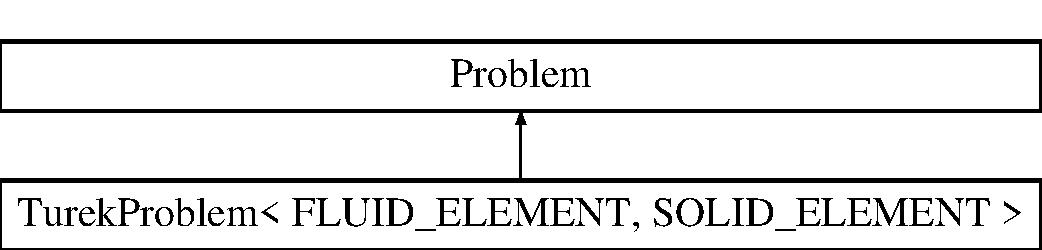
\includegraphics[height=2.000000cm]{classTurekProblem}
\end{center}
\end{figure}
\subsection*{Public Member Functions}
\begin{DoxyCompactItemize}
\item 
\hyperlink{classTurekProblem_a69f6624fd854393f0c0e5303603ec749}{Turek\+Problem} (const double \&length, const double \&height)
\begin{DoxyCompactList}\small\item\em Constructor\+: Pass length and height of domain. \end{DoxyCompactList}\item 
Refineable\+Algebraic\+Cylinder\+With\+Flag\+Mesh$<$ F\+L\+U\+I\+D\+\_\+\+E\+L\+E\+M\+E\+NT $>$ $\ast$ \hyperlink{classTurekProblem_a0fc23b86efec256cb7f4450a928f7999}{fluid\+\_\+mesh\+\_\+pt} ()
\begin{DoxyCompactList}\small\item\em Access function for the fluid mesh. \end{DoxyCompactList}\item 
Elastic\+Refineable\+Rectangular\+Quad\+Mesh$<$ S\+O\+L\+I\+D\+\_\+\+E\+L\+E\+M\+E\+NT $>$ $\ast$\& \hyperlink{classTurekProblem_a89430ae6d87a85a83e23e14e0b0d72b7}{solid\+\_\+mesh\+\_\+pt} ()
\begin{DoxyCompactList}\small\item\em Access function for the solid mesh. \end{DoxyCompactList}\item 
Solid\+Mesh $\ast$\& \hyperlink{classTurekProblem_a93a4b3d4e598a499631e00cfa701ee3c}{traction\+\_\+mesh\+\_\+pt} (const unsigned \&i)
\begin{DoxyCompactList}\small\item\em Access function for the i-\/th mesh of F\+SI traction elements. \end{DoxyCompactList}\item 
void \hyperlink{classTurekProblem_a39df0332d7606a5befe89bb0e581184b}{actions\+\_\+after\+\_\+adapt} ()
\begin{DoxyCompactList}\small\item\em Actions after adapt\+: Re-\/setup the fsi lookup scheme. \end{DoxyCompactList}\item 
void \hyperlink{classTurekProblem_a2cf0eb1610b4c3a7cdbd3c7948cdd46e}{doc\+\_\+solution} (Doc\+Info \&doc\+\_\+info, ofstream \&trace\+\_\+file)
\begin{DoxyCompactList}\small\item\em Doc the solution. \end{DoxyCompactList}\item 
void \hyperlink{classTurekProblem_ae97d3bad44e12274168e883c966b3983}{actions\+\_\+after\+\_\+newton\+\_\+solve} ()
\begin{DoxyCompactList}\small\item\em Update function (empty) \end{DoxyCompactList}\item 
void \hyperlink{classTurekProblem_a889518fdaf0c4215e21981afbfc669bd}{actions\+\_\+before\+\_\+newton\+\_\+solve} ()
\begin{DoxyCompactList}\small\item\em Update function (empty) \end{DoxyCompactList}\item 
void \hyperlink{classTurekProblem_aa896171b1a817ca35cba9b723bb15ed2}{actions\+\_\+before\+\_\+newton\+\_\+convergence\+\_\+check} ()
\begin{DoxyCompactList}\small\item\em Update the (enslaved) fluid node positions following the update of the solid variables before performing Newton convergence check. \end{DoxyCompactList}\item 
void \hyperlink{classTurekProblem_a4ad226ceec27cb3c3ea4d1ecfd4e573f}{actions\+\_\+before\+\_\+implicit\+\_\+timestep} ()
\begin{DoxyCompactList}\small\item\em Update the time-\/dependent influx. \end{DoxyCompactList}\end{DoxyCompactItemize}
\subsection*{Private Member Functions}
\begin{DoxyCompactItemize}
\item 
void \hyperlink{classTurekProblem_ad460a2e860c9425297cf70ee125de10b}{create\+\_\+fsi\+\_\+traction\+\_\+elements} ()
\begin{DoxyCompactList}\small\item\em Create F\+SI traction elements. \end{DoxyCompactList}\end{DoxyCompactItemize}
\subsection*{Private Attributes}
\begin{DoxyCompactItemize}
\item 
Elastic\+Refineable\+Rectangular\+Quad\+Mesh$<$ S\+O\+L\+I\+D\+\_\+\+E\+L\+E\+M\+E\+NT $>$ $\ast$ \hyperlink{classTurekProblem_a1a449088ae3cc96ade1c58979294afed}{Solid\+\_\+mesh\+\_\+pt}
\begin{DoxyCompactList}\small\item\em Pointer to solid mesh. \end{DoxyCompactList}\item 
Refineable\+Algebraic\+Cylinder\+With\+Flag\+Mesh$<$ F\+L\+U\+I\+D\+\_\+\+E\+L\+E\+M\+E\+NT $>$ $\ast$ \hyperlink{classTurekProblem_a18a0daace5dc50db4b93879e4a600e6a}{Fluid\+\_\+mesh\+\_\+pt}
\begin{DoxyCompactList}\small\item\em Pointer to fluid mesh. \end{DoxyCompactList}\item 
Vector$<$ Solid\+Mesh $\ast$ $>$ \hyperlink{classTurekProblem_a0b8588d0f133ffb9a281c5747786f95f}{Traction\+\_\+mesh\+\_\+pt}
\begin{DoxyCompactList}\small\item\em Vector of pointers to mesh of F\+SI traction elements. \end{DoxyCompactList}\item 
Solid\+Mesh $\ast$ \hyperlink{classTurekProblem_ac61477b19dfaaba6fb2c7a5c72240ac6}{Combined\+\_\+traction\+\_\+mesh\+\_\+pt}
\begin{DoxyCompactList}\small\item\em Combined mesh of traction elements -- only used for documentation. \end{DoxyCompactList}\item 
double \hyperlink{classTurekProblem_a24d68af05e815f7164e30f53ce7357ce}{Domain\+\_\+height}
\begin{DoxyCompactList}\small\item\em Overall height of domain. \end{DoxyCompactList}\item 
double \hyperlink{classTurekProblem_aff485942ff327ccfcafd3608910ef635}{Domain\+\_\+length}
\begin{DoxyCompactList}\small\item\em Overall length of domain. \end{DoxyCompactList}\item 
Node $\ast$ \hyperlink{classTurekProblem_ad65b9a2f833ed9bae3520980c76d1f2f}{Solid\+\_\+control\+\_\+node\+\_\+pt}
\begin{DoxyCompactList}\small\item\em Pointer to solid control node. \end{DoxyCompactList}\item 
Node $\ast$ \hyperlink{classTurekProblem_a3d297a52fffd79bb7083fd57c2574fff}{Fluid\+\_\+control\+\_\+node\+\_\+pt}
\begin{DoxyCompactList}\small\item\em Pointer to fluid control node. \end{DoxyCompactList}\end{DoxyCompactItemize}


\subsection{Detailed Description}
\subsubsection*{template$<$class F\+L\+U\+I\+D\+\_\+\+E\+L\+E\+M\+E\+NT, class S\+O\+L\+I\+D\+\_\+\+E\+L\+E\+M\+E\+NT$>$\newline
class Turek\+Problem$<$ F\+L\+U\+I\+D\+\_\+\+E\+L\+E\+M\+E\+N\+T, S\+O\+L\+I\+D\+\_\+\+E\+L\+E\+M\+E\+N\+T $>$}

Problem class. 

Definition at line 374 of file turek\+\_\+flag.\+cc.



\subsection{Constructor \& Destructor Documentation}
\mbox{\Hypertarget{classTurekProblem_a69f6624fd854393f0c0e5303603ec749}\label{classTurekProblem_a69f6624fd854393f0c0e5303603ec749}} 
\index{Turek\+Problem@{Turek\+Problem}!Turek\+Problem@{Turek\+Problem}}
\index{Turek\+Problem@{Turek\+Problem}!Turek\+Problem@{Turek\+Problem}}
\subsubsection{\texorpdfstring{Turek\+Problem()}{TurekProblem()}}
{\footnotesize\ttfamily template$<$class F\+L\+U\+I\+D\+\_\+\+E\+L\+E\+M\+E\+NT , class S\+O\+L\+I\+D\+\_\+\+E\+L\+E\+M\+E\+NT $>$ \\
\hyperlink{classTurekProblem}{Turek\+Problem}$<$ F\+L\+U\+I\+D\+\_\+\+E\+L\+E\+M\+E\+NT, S\+O\+L\+I\+D\+\_\+\+E\+L\+E\+M\+E\+NT $>$\+::\hyperlink{classTurekProblem}{Turek\+Problem} (\begin{DoxyParamCaption}\item[{const double \&}]{length,  }\item[{const double \&}]{height }\end{DoxyParamCaption})}



Constructor\+: Pass length and height of domain. 

Left point on centreline of flag so that the top and bottom vertices merge with the cylinder. 

Definition at line 451 of file turek\+\_\+flag.\+cc.



References Turek\+Problem$<$ F\+L\+U\+I\+D\+\_\+\+E\+L\+E\+M\+E\+N\+T, S\+O\+L\+I\+D\+\_\+\+E\+L\+E\+M\+E\+N\+T $>$\+::actions\+\_\+before\+\_\+newton\+\_\+convergence\+\_\+check(), Global\+\_\+\+Parameters\+::\+Centre\+\_\+x, Global\+\_\+\+Parameters\+::\+Centre\+\_\+y, Global\+\_\+\+Parameters\+::\+Constitutive\+\_\+law\+\_\+pt, Turek\+Problem$<$ F\+L\+U\+I\+D\+\_\+\+E\+L\+E\+M\+E\+N\+T, S\+O\+L\+I\+D\+\_\+\+E\+L\+E\+M\+E\+N\+T $>$\+::create\+\_\+fsi\+\_\+traction\+\_\+elements(), Turek\+Problem$<$ F\+L\+U\+I\+D\+\_\+\+E\+L\+E\+M\+E\+N\+T, S\+O\+L\+I\+D\+\_\+\+E\+L\+E\+M\+E\+N\+T $>$\+::\+Domain\+\_\+height, Turek\+Problem$<$ F\+L\+U\+I\+D\+\_\+\+E\+L\+E\+M\+E\+N\+T, S\+O\+L\+I\+D\+\_\+\+E\+L\+E\+M\+E\+N\+T $>$\+::\+Fluid\+\_\+control\+\_\+node\+\_\+pt, Turek\+Problem$<$ F\+L\+U\+I\+D\+\_\+\+E\+L\+E\+M\+E\+N\+T, S\+O\+L\+I\+D\+\_\+\+E\+L\+E\+M\+E\+N\+T $>$\+::fluid\+\_\+mesh\+\_\+pt(), Turek\+Problem$<$ F\+L\+U\+I\+D\+\_\+\+E\+L\+E\+M\+E\+N\+T, S\+O\+L\+I\+D\+\_\+\+E\+L\+E\+M\+E\+N\+T $>$\+::\+Fluid\+\_\+mesh\+\_\+pt, Global\+\_\+\+Parameters\+::flux(), Global\+\_\+\+Parameters\+::gravity(), Global\+\_\+\+Parameters\+::H, Global\+\_\+\+Parameters\+::\+Ignore\+\_\+fluid\+\_\+loading, Global\+\_\+\+Parameters\+::\+Lambda\+\_\+sq, Global\+\_\+\+Parameters\+::Q, Global\+\_\+\+Parameters\+::\+Radius, Global\+\_\+\+Parameters\+::\+Re, Global\+\_\+\+Parameters\+::\+Re\+St, Turek\+Problem$<$ F\+L\+U\+I\+D\+\_\+\+E\+L\+E\+M\+E\+N\+T, S\+O\+L\+I\+D\+\_\+\+E\+L\+E\+M\+E\+N\+T $>$\+::\+Solid\+\_\+control\+\_\+node\+\_\+pt, Turek\+Problem$<$ F\+L\+U\+I\+D\+\_\+\+E\+L\+E\+M\+E\+N\+T, S\+O\+L\+I\+D\+\_\+\+E\+L\+E\+M\+E\+N\+T $>$\+::solid\+\_\+mesh\+\_\+pt(), Global\+\_\+\+Parameters\+::\+St, Turek\+Problem$<$ F\+L\+U\+I\+D\+\_\+\+E\+L\+E\+M\+E\+N\+T, S\+O\+L\+I\+D\+\_\+\+E\+L\+E\+M\+E\+N\+T $>$\+::traction\+\_\+mesh\+\_\+pt(), and Turek\+Problem$<$ F\+L\+U\+I\+D\+\_\+\+E\+L\+E\+M\+E\+N\+T, S\+O\+L\+I\+D\+\_\+\+E\+L\+E\+M\+E\+N\+T $>$\+::\+Traction\+\_\+mesh\+\_\+pt.



\subsection{Member Function Documentation}
\mbox{\Hypertarget{classTurekProblem_a39df0332d7606a5befe89bb0e581184b}\label{classTurekProblem_a39df0332d7606a5befe89bb0e581184b}} 
\index{Turek\+Problem@{Turek\+Problem}!actions\+\_\+after\+\_\+adapt@{actions\+\_\+after\+\_\+adapt}}
\index{actions\+\_\+after\+\_\+adapt@{actions\+\_\+after\+\_\+adapt}!Turek\+Problem@{Turek\+Problem}}
\subsubsection{\texorpdfstring{actions\+\_\+after\+\_\+adapt()}{actions\_after\_adapt()}}
{\footnotesize\ttfamily template$<$class F\+L\+U\+I\+D\+\_\+\+E\+L\+E\+M\+E\+NT , class S\+O\+L\+I\+D\+\_\+\+E\+L\+E\+M\+E\+NT $>$ \\
void \hyperlink{classTurekProblem}{Turek\+Problem}$<$ F\+L\+U\+I\+D\+\_\+\+E\+L\+E\+M\+E\+NT, S\+O\+L\+I\+D\+\_\+\+E\+L\+E\+M\+E\+NT $>$\+::actions\+\_\+after\+\_\+adapt (\begin{DoxyParamCaption}{ }\end{DoxyParamCaption})}



Actions after adapt\+: Re-\/setup the fsi lookup scheme. 

Actions after adapt\+: Re-\/setup F\+SI. 

Definition at line 899 of file turek\+\_\+flag.\+cc.



References Turek\+Problem$<$ F\+L\+U\+I\+D\+\_\+\+E\+L\+E\+M\+E\+N\+T, S\+O\+L\+I\+D\+\_\+\+E\+L\+E\+M\+E\+N\+T $>$\+::fluid\+\_\+mesh\+\_\+pt(), Turek\+Problem$<$ F\+L\+U\+I\+D\+\_\+\+E\+L\+E\+M\+E\+N\+T, S\+O\+L\+I\+D\+\_\+\+E\+L\+E\+M\+E\+N\+T $>$\+::\+Fluid\+\_\+mesh\+\_\+pt, Global\+\_\+\+Parameters\+::\+Ignore\+\_\+fluid\+\_\+loading, Turek\+Problem$<$ F\+L\+U\+I\+D\+\_\+\+E\+L\+E\+M\+E\+N\+T, S\+O\+L\+I\+D\+\_\+\+E\+L\+E\+M\+E\+N\+T $>$\+::solid\+\_\+mesh\+\_\+pt(), and Turek\+Problem$<$ F\+L\+U\+I\+D\+\_\+\+E\+L\+E\+M\+E\+N\+T, S\+O\+L\+I\+D\+\_\+\+E\+L\+E\+M\+E\+N\+T $>$\+::\+Traction\+\_\+mesh\+\_\+pt.

\mbox{\Hypertarget{classTurekProblem_ae97d3bad44e12274168e883c966b3983}\label{classTurekProblem_ae97d3bad44e12274168e883c966b3983}} 
\index{Turek\+Problem@{Turek\+Problem}!actions\+\_\+after\+\_\+newton\+\_\+solve@{actions\+\_\+after\+\_\+newton\+\_\+solve}}
\index{actions\+\_\+after\+\_\+newton\+\_\+solve@{actions\+\_\+after\+\_\+newton\+\_\+solve}!Turek\+Problem@{Turek\+Problem}}
\subsubsection{\texorpdfstring{actions\+\_\+after\+\_\+newton\+\_\+solve()}{actions\_after\_newton\_solve()}}
{\footnotesize\ttfamily template$<$class F\+L\+U\+I\+D\+\_\+\+E\+L\+E\+M\+E\+NT, class S\+O\+L\+I\+D\+\_\+\+E\+L\+E\+M\+E\+NT$>$ \\
void \hyperlink{classTurekProblem}{Turek\+Problem}$<$ F\+L\+U\+I\+D\+\_\+\+E\+L\+E\+M\+E\+NT, S\+O\+L\+I\+D\+\_\+\+E\+L\+E\+M\+E\+NT $>$\+::actions\+\_\+after\+\_\+newton\+\_\+solve (\begin{DoxyParamCaption}{ }\end{DoxyParamCaption})\hspace{0.3cm}{\ttfamily [inline]}}



Update function (empty) 



Definition at line 401 of file turek\+\_\+flag.\+cc.

\mbox{\Hypertarget{classTurekProblem_a4ad226ceec27cb3c3ea4d1ecfd4e573f}\label{classTurekProblem_a4ad226ceec27cb3c3ea4d1ecfd4e573f}} 
\index{Turek\+Problem@{Turek\+Problem}!actions\+\_\+before\+\_\+implicit\+\_\+timestep@{actions\+\_\+before\+\_\+implicit\+\_\+timestep}}
\index{actions\+\_\+before\+\_\+implicit\+\_\+timestep@{actions\+\_\+before\+\_\+implicit\+\_\+timestep}!Turek\+Problem@{Turek\+Problem}}
\subsubsection{\texorpdfstring{actions\+\_\+before\+\_\+implicit\+\_\+timestep()}{actions\_before\_implicit\_timestep()}}
{\footnotesize\ttfamily template$<$class F\+L\+U\+I\+D\+\_\+\+E\+L\+E\+M\+E\+NT , class S\+O\+L\+I\+D\+\_\+\+E\+L\+E\+M\+E\+NT $>$ \\
void \hyperlink{classTurekProblem}{Turek\+Problem}$<$ F\+L\+U\+I\+D\+\_\+\+E\+L\+E\+M\+E\+NT, S\+O\+L\+I\+D\+\_\+\+E\+L\+E\+M\+E\+NT $>$\+::actions\+\_\+before\+\_\+implicit\+\_\+timestep (\begin{DoxyParamCaption}{ }\end{DoxyParamCaption})}



Update the time-\/dependent influx. 

Actions before implicit timestep\+: Update inflow profile. 

Definition at line 873 of file turek\+\_\+flag.\+cc.



References Turek\+Problem$<$ F\+L\+U\+I\+D\+\_\+\+E\+L\+E\+M\+E\+N\+T, S\+O\+L\+I\+D\+\_\+\+E\+L\+E\+M\+E\+N\+T $>$\+::\+Domain\+\_\+height, Turek\+Problem$<$ F\+L\+U\+I\+D\+\_\+\+E\+L\+E\+M\+E\+N\+T, S\+O\+L\+I\+D\+\_\+\+E\+L\+E\+M\+E\+N\+T $>$\+::\+Fluid\+\_\+mesh\+\_\+pt, and Global\+\_\+\+Parameters\+::flux().



Referenced by Turek\+Problem$<$ F\+L\+U\+I\+D\+\_\+\+E\+L\+E\+M\+E\+N\+T, S\+O\+L\+I\+D\+\_\+\+E\+L\+E\+M\+E\+N\+T $>$\+::actions\+\_\+before\+\_\+newton\+\_\+convergence\+\_\+check().

\mbox{\Hypertarget{classTurekProblem_aa896171b1a817ca35cba9b723bb15ed2}\label{classTurekProblem_aa896171b1a817ca35cba9b723bb15ed2}} 
\index{Turek\+Problem@{Turek\+Problem}!actions\+\_\+before\+\_\+newton\+\_\+convergence\+\_\+check@{actions\+\_\+before\+\_\+newton\+\_\+convergence\+\_\+check}}
\index{actions\+\_\+before\+\_\+newton\+\_\+convergence\+\_\+check@{actions\+\_\+before\+\_\+newton\+\_\+convergence\+\_\+check}!Turek\+Problem@{Turek\+Problem}}
\subsubsection{\texorpdfstring{actions\+\_\+before\+\_\+newton\+\_\+convergence\+\_\+check()}{actions\_before\_newton\_convergence\_check()}}
{\footnotesize\ttfamily template$<$class F\+L\+U\+I\+D\+\_\+\+E\+L\+E\+M\+E\+NT , class S\+O\+L\+I\+D\+\_\+\+E\+L\+E\+M\+E\+NT $>$ \\
void \hyperlink{classTurekProblem}{Turek\+Problem}$<$ F\+L\+U\+I\+D\+\_\+\+E\+L\+E\+M\+E\+NT, S\+O\+L\+I\+D\+\_\+\+E\+L\+E\+M\+E\+NT $>$\+::actions\+\_\+before\+\_\+newton\+\_\+convergence\+\_\+check (\begin{DoxyParamCaption}{ }\end{DoxyParamCaption})}



Update the (enslaved) fluid node positions following the update of the solid variables before performing Newton convergence check. 

Update the (enslaved) fluid node positions following the update of the solid variables 

Definition at line 861 of file turek\+\_\+flag.\+cc.



References Turek\+Problem$<$ F\+L\+U\+I\+D\+\_\+\+E\+L\+E\+M\+E\+N\+T, S\+O\+L\+I\+D\+\_\+\+E\+L\+E\+M\+E\+N\+T $>$\+::actions\+\_\+before\+\_\+implicit\+\_\+timestep(), and Turek\+Problem$<$ F\+L\+U\+I\+D\+\_\+\+E\+L\+E\+M\+E\+N\+T, S\+O\+L\+I\+D\+\_\+\+E\+L\+E\+M\+E\+N\+T $>$\+::fluid\+\_\+mesh\+\_\+pt().



Referenced by Turek\+Problem$<$ F\+L\+U\+I\+D\+\_\+\+E\+L\+E\+M\+E\+N\+T, S\+O\+L\+I\+D\+\_\+\+E\+L\+E\+M\+E\+N\+T $>$\+::\+Turek\+Problem().

\mbox{\Hypertarget{classTurekProblem_a889518fdaf0c4215e21981afbfc669bd}\label{classTurekProblem_a889518fdaf0c4215e21981afbfc669bd}} 
\index{Turek\+Problem@{Turek\+Problem}!actions\+\_\+before\+\_\+newton\+\_\+solve@{actions\+\_\+before\+\_\+newton\+\_\+solve}}
\index{actions\+\_\+before\+\_\+newton\+\_\+solve@{actions\+\_\+before\+\_\+newton\+\_\+solve}!Turek\+Problem@{Turek\+Problem}}
\subsubsection{\texorpdfstring{actions\+\_\+before\+\_\+newton\+\_\+solve()}{actions\_before\_newton\_solve()}}
{\footnotesize\ttfamily template$<$class F\+L\+U\+I\+D\+\_\+\+E\+L\+E\+M\+E\+NT, class S\+O\+L\+I\+D\+\_\+\+E\+L\+E\+M\+E\+NT$>$ \\
void \hyperlink{classTurekProblem}{Turek\+Problem}$<$ F\+L\+U\+I\+D\+\_\+\+E\+L\+E\+M\+E\+NT, S\+O\+L\+I\+D\+\_\+\+E\+L\+E\+M\+E\+NT $>$\+::actions\+\_\+before\+\_\+newton\+\_\+solve (\begin{DoxyParamCaption}{ }\end{DoxyParamCaption})\hspace{0.3cm}{\ttfamily [inline]}}



Update function (empty) 



Definition at line 404 of file turek\+\_\+flag.\+cc.

\mbox{\Hypertarget{classTurekProblem_ad460a2e860c9425297cf70ee125de10b}\label{classTurekProblem_ad460a2e860c9425297cf70ee125de10b}} 
\index{Turek\+Problem@{Turek\+Problem}!create\+\_\+fsi\+\_\+traction\+\_\+elements@{create\+\_\+fsi\+\_\+traction\+\_\+elements}}
\index{create\+\_\+fsi\+\_\+traction\+\_\+elements@{create\+\_\+fsi\+\_\+traction\+\_\+elements}!Turek\+Problem@{Turek\+Problem}}
\subsubsection{\texorpdfstring{create\+\_\+fsi\+\_\+traction\+\_\+elements()}{create\_fsi\_traction\_elements()}}
{\footnotesize\ttfamily template$<$class F\+L\+U\+I\+D\+\_\+\+E\+L\+E\+M\+E\+NT , class S\+O\+L\+I\+D\+\_\+\+E\+L\+E\+M\+E\+NT $>$ \\
void \hyperlink{classTurekProblem}{Turek\+Problem}$<$ F\+L\+U\+I\+D\+\_\+\+E\+L\+E\+M\+E\+NT, S\+O\+L\+I\+D\+\_\+\+E\+L\+E\+M\+E\+NT $>$\+::create\+\_\+fsi\+\_\+traction\+\_\+elements (\begin{DoxyParamCaption}{ }\end{DoxyParamCaption})\hspace{0.3cm}{\ttfamily [private]}}



Create F\+SI traction elements. 



Definition at line 957 of file turek\+\_\+flag.\+cc.



References Turek\+Problem$<$ F\+L\+U\+I\+D\+\_\+\+E\+L\+E\+M\+E\+N\+T, S\+O\+L\+I\+D\+\_\+\+E\+L\+E\+M\+E\+N\+T $>$\+::\+Combined\+\_\+traction\+\_\+mesh\+\_\+pt, Turek\+Problem$<$ F\+L\+U\+I\+D\+\_\+\+E\+L\+E\+M\+E\+N\+T, S\+O\+L\+I\+D\+\_\+\+E\+L\+E\+M\+E\+N\+T $>$\+::solid\+\_\+mesh\+\_\+pt(), and Turek\+Problem$<$ F\+L\+U\+I\+D\+\_\+\+E\+L\+E\+M\+E\+N\+T, S\+O\+L\+I\+D\+\_\+\+E\+L\+E\+M\+E\+N\+T $>$\+::\+Traction\+\_\+mesh\+\_\+pt.



Referenced by Turek\+Problem$<$ F\+L\+U\+I\+D\+\_\+\+E\+L\+E\+M\+E\+N\+T, S\+O\+L\+I\+D\+\_\+\+E\+L\+E\+M\+E\+N\+T $>$\+::\+Turek\+Problem().

\mbox{\Hypertarget{classTurekProblem_a2cf0eb1610b4c3a7cdbd3c7948cdd46e}\label{classTurekProblem_a2cf0eb1610b4c3a7cdbd3c7948cdd46e}} 
\index{Turek\+Problem@{Turek\+Problem}!doc\+\_\+solution@{doc\+\_\+solution}}
\index{doc\+\_\+solution@{doc\+\_\+solution}!Turek\+Problem@{Turek\+Problem}}
\subsubsection{\texorpdfstring{doc\+\_\+solution()}{doc\_solution()}}
{\footnotesize\ttfamily template$<$class F\+L\+U\+I\+D\+\_\+\+E\+L\+E\+M\+E\+NT , class S\+O\+L\+I\+D\+\_\+\+E\+L\+E\+M\+E\+NT $>$ \\
void \hyperlink{classTurekProblem}{Turek\+Problem}$<$ F\+L\+U\+I\+D\+\_\+\+E\+L\+E\+M\+E\+NT, S\+O\+L\+I\+D\+\_\+\+E\+L\+E\+M\+E\+NT $>$\+::doc\+\_\+solution (\begin{DoxyParamCaption}\item[{Doc\+Info \&}]{doc\+\_\+info,  }\item[{ofstream \&}]{trace\+\_\+file }\end{DoxyParamCaption})}



Doc the solution. 



Definition at line 1012 of file turek\+\_\+flag.\+cc.



References Turek\+Problem$<$ F\+L\+U\+I\+D\+\_\+\+E\+L\+E\+M\+E\+N\+T, S\+O\+L\+I\+D\+\_\+\+E\+L\+E\+M\+E\+N\+T $>$\+::\+Fluid\+\_\+control\+\_\+node\+\_\+pt, Turek\+Problem$<$ F\+L\+U\+I\+D\+\_\+\+E\+L\+E\+M\+E\+N\+T, S\+O\+L\+I\+D\+\_\+\+E\+L\+E\+M\+E\+N\+T $>$\+::fluid\+\_\+mesh\+\_\+pt(), Global\+\_\+\+Parameters\+::flux(), Turek\+Problem$<$ F\+L\+U\+I\+D\+\_\+\+E\+L\+E\+M\+E\+N\+T, S\+O\+L\+I\+D\+\_\+\+E\+L\+E\+M\+E\+N\+T $>$\+::\+Solid\+\_\+control\+\_\+node\+\_\+pt, Turek\+Problem$<$ F\+L\+U\+I\+D\+\_\+\+E\+L\+E\+M\+E\+N\+T, S\+O\+L\+I\+D\+\_\+\+E\+L\+E\+M\+E\+N\+T $>$\+::solid\+\_\+mesh\+\_\+pt(), and Turek\+Problem$<$ F\+L\+U\+I\+D\+\_\+\+E\+L\+E\+M\+E\+N\+T, S\+O\+L\+I\+D\+\_\+\+E\+L\+E\+M\+E\+N\+T $>$\+::\+Traction\+\_\+mesh\+\_\+pt.



Referenced by main().

\mbox{\Hypertarget{classTurekProblem_a0fc23b86efec256cb7f4450a928f7999}\label{classTurekProblem_a0fc23b86efec256cb7f4450a928f7999}} 
\index{Turek\+Problem@{Turek\+Problem}!fluid\+\_\+mesh\+\_\+pt@{fluid\+\_\+mesh\+\_\+pt}}
\index{fluid\+\_\+mesh\+\_\+pt@{fluid\+\_\+mesh\+\_\+pt}!Turek\+Problem@{Turek\+Problem}}
\subsubsection{\texorpdfstring{fluid\+\_\+mesh\+\_\+pt()}{fluid\_mesh\_pt()}}
{\footnotesize\ttfamily template$<$class F\+L\+U\+I\+D\+\_\+\+E\+L\+E\+M\+E\+NT, class S\+O\+L\+I\+D\+\_\+\+E\+L\+E\+M\+E\+NT$>$ \\
Refineable\+Algebraic\+Cylinder\+With\+Flag\+Mesh$<$F\+L\+U\+I\+D\+\_\+\+E\+L\+E\+M\+E\+NT$>$$\ast$ \hyperlink{classTurekProblem}{Turek\+Problem}$<$ F\+L\+U\+I\+D\+\_\+\+E\+L\+E\+M\+E\+NT, S\+O\+L\+I\+D\+\_\+\+E\+L\+E\+M\+E\+NT $>$\+::fluid\+\_\+mesh\+\_\+pt (\begin{DoxyParamCaption}{ }\end{DoxyParamCaption})\hspace{0.3cm}{\ttfamily [inline]}}



Access function for the fluid mesh. 



Definition at line 383 of file turek\+\_\+flag.\+cc.



Referenced by Turek\+Problem$<$ F\+L\+U\+I\+D\+\_\+\+E\+L\+E\+M\+E\+N\+T, S\+O\+L\+I\+D\+\_\+\+E\+L\+E\+M\+E\+N\+T $>$\+::actions\+\_\+after\+\_\+adapt(), Turek\+Problem$<$ F\+L\+U\+I\+D\+\_\+\+E\+L\+E\+M\+E\+N\+T, S\+O\+L\+I\+D\+\_\+\+E\+L\+E\+M\+E\+N\+T $>$\+::actions\+\_\+before\+\_\+newton\+\_\+convergence\+\_\+check(), Turek\+Problem$<$ F\+L\+U\+I\+D\+\_\+\+E\+L\+E\+M\+E\+N\+T, S\+O\+L\+I\+D\+\_\+\+E\+L\+E\+M\+E\+N\+T $>$\+::doc\+\_\+solution(), and Turek\+Problem$<$ F\+L\+U\+I\+D\+\_\+\+E\+L\+E\+M\+E\+N\+T, S\+O\+L\+I\+D\+\_\+\+E\+L\+E\+M\+E\+N\+T $>$\+::\+Turek\+Problem().

\mbox{\Hypertarget{classTurekProblem_a89430ae6d87a85a83e23e14e0b0d72b7}\label{classTurekProblem_a89430ae6d87a85a83e23e14e0b0d72b7}} 
\index{Turek\+Problem@{Turek\+Problem}!solid\+\_\+mesh\+\_\+pt@{solid\+\_\+mesh\+\_\+pt}}
\index{solid\+\_\+mesh\+\_\+pt@{solid\+\_\+mesh\+\_\+pt}!Turek\+Problem@{Turek\+Problem}}
\subsubsection{\texorpdfstring{solid\+\_\+mesh\+\_\+pt()}{solid\_mesh\_pt()}}
{\footnotesize\ttfamily template$<$class F\+L\+U\+I\+D\+\_\+\+E\+L\+E\+M\+E\+NT, class S\+O\+L\+I\+D\+\_\+\+E\+L\+E\+M\+E\+NT$>$ \\
Elastic\+Refineable\+Rectangular\+Quad\+Mesh$<$S\+O\+L\+I\+D\+\_\+\+E\+L\+E\+M\+E\+NT$>$$\ast$\& \hyperlink{classTurekProblem}{Turek\+Problem}$<$ F\+L\+U\+I\+D\+\_\+\+E\+L\+E\+M\+E\+NT, S\+O\+L\+I\+D\+\_\+\+E\+L\+E\+M\+E\+NT $>$\+::solid\+\_\+mesh\+\_\+pt (\begin{DoxyParamCaption}{ }\end{DoxyParamCaption})\hspace{0.3cm}{\ttfamily [inline]}}



Access function for the solid mesh. 



Definition at line 387 of file turek\+\_\+flag.\+cc.



Referenced by Turek\+Problem$<$ F\+L\+U\+I\+D\+\_\+\+E\+L\+E\+M\+E\+N\+T, S\+O\+L\+I\+D\+\_\+\+E\+L\+E\+M\+E\+N\+T $>$\+::actions\+\_\+after\+\_\+adapt(), Turek\+Problem$<$ F\+L\+U\+I\+D\+\_\+\+E\+L\+E\+M\+E\+N\+T, S\+O\+L\+I\+D\+\_\+\+E\+L\+E\+M\+E\+N\+T $>$\+::create\+\_\+fsi\+\_\+traction\+\_\+elements(), Turek\+Problem$<$ F\+L\+U\+I\+D\+\_\+\+E\+L\+E\+M\+E\+N\+T, S\+O\+L\+I\+D\+\_\+\+E\+L\+E\+M\+E\+N\+T $>$\+::doc\+\_\+solution(), and Turek\+Problem$<$ F\+L\+U\+I\+D\+\_\+\+E\+L\+E\+M\+E\+N\+T, S\+O\+L\+I\+D\+\_\+\+E\+L\+E\+M\+E\+N\+T $>$\+::\+Turek\+Problem().

\mbox{\Hypertarget{classTurekProblem_a93a4b3d4e598a499631e00cfa701ee3c}\label{classTurekProblem_a93a4b3d4e598a499631e00cfa701ee3c}} 
\index{Turek\+Problem@{Turek\+Problem}!traction\+\_\+mesh\+\_\+pt@{traction\+\_\+mesh\+\_\+pt}}
\index{traction\+\_\+mesh\+\_\+pt@{traction\+\_\+mesh\+\_\+pt}!Turek\+Problem@{Turek\+Problem}}
\subsubsection{\texorpdfstring{traction\+\_\+mesh\+\_\+pt()}{traction\_mesh\_pt()}}
{\footnotesize\ttfamily template$<$class F\+L\+U\+I\+D\+\_\+\+E\+L\+E\+M\+E\+NT, class S\+O\+L\+I\+D\+\_\+\+E\+L\+E\+M\+E\+NT$>$ \\
Solid\+Mesh$\ast$\& \hyperlink{classTurekProblem}{Turek\+Problem}$<$ F\+L\+U\+I\+D\+\_\+\+E\+L\+E\+M\+E\+NT, S\+O\+L\+I\+D\+\_\+\+E\+L\+E\+M\+E\+NT $>$\+::traction\+\_\+mesh\+\_\+pt (\begin{DoxyParamCaption}\item[{const unsigned \&}]{i }\end{DoxyParamCaption})\hspace{0.3cm}{\ttfamily [inline]}}



Access function for the i-\/th mesh of F\+SI traction elements. 



Definition at line 391 of file turek\+\_\+flag.\+cc.



Referenced by Turek\+Problem$<$ F\+L\+U\+I\+D\+\_\+\+E\+L\+E\+M\+E\+N\+T, S\+O\+L\+I\+D\+\_\+\+E\+L\+E\+M\+E\+N\+T $>$\+::\+Turek\+Problem().



\subsection{Member Data Documentation}
\mbox{\Hypertarget{classTurekProblem_ac61477b19dfaaba6fb2c7a5c72240ac6}\label{classTurekProblem_ac61477b19dfaaba6fb2c7a5c72240ac6}} 
\index{Turek\+Problem@{Turek\+Problem}!Combined\+\_\+traction\+\_\+mesh\+\_\+pt@{Combined\+\_\+traction\+\_\+mesh\+\_\+pt}}
\index{Combined\+\_\+traction\+\_\+mesh\+\_\+pt@{Combined\+\_\+traction\+\_\+mesh\+\_\+pt}!Turek\+Problem@{Turek\+Problem}}
\subsubsection{\texorpdfstring{Combined\+\_\+traction\+\_\+mesh\+\_\+pt}{Combined\_traction\_mesh\_pt}}
{\footnotesize\ttfamily template$<$class F\+L\+U\+I\+D\+\_\+\+E\+L\+E\+M\+E\+NT, class S\+O\+L\+I\+D\+\_\+\+E\+L\+E\+M\+E\+NT$>$ \\
Solid\+Mesh$\ast$ \hyperlink{classTurekProblem}{Turek\+Problem}$<$ F\+L\+U\+I\+D\+\_\+\+E\+L\+E\+M\+E\+NT, S\+O\+L\+I\+D\+\_\+\+E\+L\+E\+M\+E\+NT $>$\+::Combined\+\_\+traction\+\_\+mesh\+\_\+pt\hspace{0.3cm}{\ttfamily [private]}}



Combined mesh of traction elements -- only used for documentation. 



Definition at line 429 of file turek\+\_\+flag.\+cc.



Referenced by Turek\+Problem$<$ F\+L\+U\+I\+D\+\_\+\+E\+L\+E\+M\+E\+N\+T, S\+O\+L\+I\+D\+\_\+\+E\+L\+E\+M\+E\+N\+T $>$\+::create\+\_\+fsi\+\_\+traction\+\_\+elements().

\mbox{\Hypertarget{classTurekProblem_a24d68af05e815f7164e30f53ce7357ce}\label{classTurekProblem_a24d68af05e815f7164e30f53ce7357ce}} 
\index{Turek\+Problem@{Turek\+Problem}!Domain\+\_\+height@{Domain\+\_\+height}}
\index{Domain\+\_\+height@{Domain\+\_\+height}!Turek\+Problem@{Turek\+Problem}}
\subsubsection{\texorpdfstring{Domain\+\_\+height}{Domain\_height}}
{\footnotesize\ttfamily template$<$class F\+L\+U\+I\+D\+\_\+\+E\+L\+E\+M\+E\+NT, class S\+O\+L\+I\+D\+\_\+\+E\+L\+E\+M\+E\+NT$>$ \\
double \hyperlink{classTurekProblem}{Turek\+Problem}$<$ F\+L\+U\+I\+D\+\_\+\+E\+L\+E\+M\+E\+NT, S\+O\+L\+I\+D\+\_\+\+E\+L\+E\+M\+E\+NT $>$\+::Domain\+\_\+height\hspace{0.3cm}{\ttfamily [private]}}



Overall height of domain. 



Definition at line 432 of file turek\+\_\+flag.\+cc.



Referenced by Turek\+Problem$<$ F\+L\+U\+I\+D\+\_\+\+E\+L\+E\+M\+E\+N\+T, S\+O\+L\+I\+D\+\_\+\+E\+L\+E\+M\+E\+N\+T $>$\+::actions\+\_\+before\+\_\+implicit\+\_\+timestep(), and Turek\+Problem$<$ F\+L\+U\+I\+D\+\_\+\+E\+L\+E\+M\+E\+N\+T, S\+O\+L\+I\+D\+\_\+\+E\+L\+E\+M\+E\+N\+T $>$\+::\+Turek\+Problem().

\mbox{\Hypertarget{classTurekProblem_aff485942ff327ccfcafd3608910ef635}\label{classTurekProblem_aff485942ff327ccfcafd3608910ef635}} 
\index{Turek\+Problem@{Turek\+Problem}!Domain\+\_\+length@{Domain\+\_\+length}}
\index{Domain\+\_\+length@{Domain\+\_\+length}!Turek\+Problem@{Turek\+Problem}}
\subsubsection{\texorpdfstring{Domain\+\_\+length}{Domain\_length}}
{\footnotesize\ttfamily template$<$class F\+L\+U\+I\+D\+\_\+\+E\+L\+E\+M\+E\+NT, class S\+O\+L\+I\+D\+\_\+\+E\+L\+E\+M\+E\+NT$>$ \\
double \hyperlink{classTurekProblem}{Turek\+Problem}$<$ F\+L\+U\+I\+D\+\_\+\+E\+L\+E\+M\+E\+NT, S\+O\+L\+I\+D\+\_\+\+E\+L\+E\+M\+E\+NT $>$\+::Domain\+\_\+length\hspace{0.3cm}{\ttfamily [private]}}



Overall length of domain. 



Definition at line 435 of file turek\+\_\+flag.\+cc.

\mbox{\Hypertarget{classTurekProblem_a3d297a52fffd79bb7083fd57c2574fff}\label{classTurekProblem_a3d297a52fffd79bb7083fd57c2574fff}} 
\index{Turek\+Problem@{Turek\+Problem}!Fluid\+\_\+control\+\_\+node\+\_\+pt@{Fluid\+\_\+control\+\_\+node\+\_\+pt}}
\index{Fluid\+\_\+control\+\_\+node\+\_\+pt@{Fluid\+\_\+control\+\_\+node\+\_\+pt}!Turek\+Problem@{Turek\+Problem}}
\subsubsection{\texorpdfstring{Fluid\+\_\+control\+\_\+node\+\_\+pt}{Fluid\_control\_node\_pt}}
{\footnotesize\ttfamily template$<$class F\+L\+U\+I\+D\+\_\+\+E\+L\+E\+M\+E\+NT, class S\+O\+L\+I\+D\+\_\+\+E\+L\+E\+M\+E\+NT$>$ \\
Node$\ast$ \hyperlink{classTurekProblem}{Turek\+Problem}$<$ F\+L\+U\+I\+D\+\_\+\+E\+L\+E\+M\+E\+NT, S\+O\+L\+I\+D\+\_\+\+E\+L\+E\+M\+E\+NT $>$\+::Fluid\+\_\+control\+\_\+node\+\_\+pt\hspace{0.3cm}{\ttfamily [private]}}



Pointer to fluid control node. 



Definition at line 441 of file turek\+\_\+flag.\+cc.



Referenced by Turek\+Problem$<$ F\+L\+U\+I\+D\+\_\+\+E\+L\+E\+M\+E\+N\+T, S\+O\+L\+I\+D\+\_\+\+E\+L\+E\+M\+E\+N\+T $>$\+::doc\+\_\+solution(), and Turek\+Problem$<$ F\+L\+U\+I\+D\+\_\+\+E\+L\+E\+M\+E\+N\+T, S\+O\+L\+I\+D\+\_\+\+E\+L\+E\+M\+E\+N\+T $>$\+::\+Turek\+Problem().

\mbox{\Hypertarget{classTurekProblem_a18a0daace5dc50db4b93879e4a600e6a}\label{classTurekProblem_a18a0daace5dc50db4b93879e4a600e6a}} 
\index{Turek\+Problem@{Turek\+Problem}!Fluid\+\_\+mesh\+\_\+pt@{Fluid\+\_\+mesh\+\_\+pt}}
\index{Fluid\+\_\+mesh\+\_\+pt@{Fluid\+\_\+mesh\+\_\+pt}!Turek\+Problem@{Turek\+Problem}}
\subsubsection{\texorpdfstring{Fluid\+\_\+mesh\+\_\+pt}{Fluid\_mesh\_pt}}
{\footnotesize\ttfamily template$<$class F\+L\+U\+I\+D\+\_\+\+E\+L\+E\+M\+E\+NT, class S\+O\+L\+I\+D\+\_\+\+E\+L\+E\+M\+E\+NT$>$ \\
Refineable\+Algebraic\+Cylinder\+With\+Flag\+Mesh$<$F\+L\+U\+I\+D\+\_\+\+E\+L\+E\+M\+E\+NT$>$$\ast$ \hyperlink{classTurekProblem}{Turek\+Problem}$<$ F\+L\+U\+I\+D\+\_\+\+E\+L\+E\+M\+E\+NT, S\+O\+L\+I\+D\+\_\+\+E\+L\+E\+M\+E\+NT $>$\+::Fluid\+\_\+mesh\+\_\+pt\hspace{0.3cm}{\ttfamily [private]}}



Pointer to fluid mesh. 



Definition at line 423 of file turek\+\_\+flag.\+cc.



Referenced by Turek\+Problem$<$ F\+L\+U\+I\+D\+\_\+\+E\+L\+E\+M\+E\+N\+T, S\+O\+L\+I\+D\+\_\+\+E\+L\+E\+M\+E\+N\+T $>$\+::actions\+\_\+after\+\_\+adapt(), Turek\+Problem$<$ F\+L\+U\+I\+D\+\_\+\+E\+L\+E\+M\+E\+N\+T, S\+O\+L\+I\+D\+\_\+\+E\+L\+E\+M\+E\+N\+T $>$\+::actions\+\_\+before\+\_\+implicit\+\_\+timestep(), and Turek\+Problem$<$ F\+L\+U\+I\+D\+\_\+\+E\+L\+E\+M\+E\+N\+T, S\+O\+L\+I\+D\+\_\+\+E\+L\+E\+M\+E\+N\+T $>$\+::\+Turek\+Problem().

\mbox{\Hypertarget{classTurekProblem_ad65b9a2f833ed9bae3520980c76d1f2f}\label{classTurekProblem_ad65b9a2f833ed9bae3520980c76d1f2f}} 
\index{Turek\+Problem@{Turek\+Problem}!Solid\+\_\+control\+\_\+node\+\_\+pt@{Solid\+\_\+control\+\_\+node\+\_\+pt}}
\index{Solid\+\_\+control\+\_\+node\+\_\+pt@{Solid\+\_\+control\+\_\+node\+\_\+pt}!Turek\+Problem@{Turek\+Problem}}
\subsubsection{\texorpdfstring{Solid\+\_\+control\+\_\+node\+\_\+pt}{Solid\_control\_node\_pt}}
{\footnotesize\ttfamily template$<$class F\+L\+U\+I\+D\+\_\+\+E\+L\+E\+M\+E\+NT, class S\+O\+L\+I\+D\+\_\+\+E\+L\+E\+M\+E\+NT$>$ \\
Node$\ast$ \hyperlink{classTurekProblem}{Turek\+Problem}$<$ F\+L\+U\+I\+D\+\_\+\+E\+L\+E\+M\+E\+NT, S\+O\+L\+I\+D\+\_\+\+E\+L\+E\+M\+E\+NT $>$\+::Solid\+\_\+control\+\_\+node\+\_\+pt\hspace{0.3cm}{\ttfamily [private]}}



Pointer to solid control node. 



Definition at line 438 of file turek\+\_\+flag.\+cc.



Referenced by Turek\+Problem$<$ F\+L\+U\+I\+D\+\_\+\+E\+L\+E\+M\+E\+N\+T, S\+O\+L\+I\+D\+\_\+\+E\+L\+E\+M\+E\+N\+T $>$\+::doc\+\_\+solution(), and Turek\+Problem$<$ F\+L\+U\+I\+D\+\_\+\+E\+L\+E\+M\+E\+N\+T, S\+O\+L\+I\+D\+\_\+\+E\+L\+E\+M\+E\+N\+T $>$\+::\+Turek\+Problem().

\mbox{\Hypertarget{classTurekProblem_a1a449088ae3cc96ade1c58979294afed}\label{classTurekProblem_a1a449088ae3cc96ade1c58979294afed}} 
\index{Turek\+Problem@{Turek\+Problem}!Solid\+\_\+mesh\+\_\+pt@{Solid\+\_\+mesh\+\_\+pt}}
\index{Solid\+\_\+mesh\+\_\+pt@{Solid\+\_\+mesh\+\_\+pt}!Turek\+Problem@{Turek\+Problem}}
\subsubsection{\texorpdfstring{Solid\+\_\+mesh\+\_\+pt}{Solid\_mesh\_pt}}
{\footnotesize\ttfamily template$<$class F\+L\+U\+I\+D\+\_\+\+E\+L\+E\+M\+E\+NT, class S\+O\+L\+I\+D\+\_\+\+E\+L\+E\+M\+E\+NT$>$ \\
Elastic\+Refineable\+Rectangular\+Quad\+Mesh$<$S\+O\+L\+I\+D\+\_\+\+E\+L\+E\+M\+E\+NT$>$$\ast$ \hyperlink{classTurekProblem}{Turek\+Problem}$<$ F\+L\+U\+I\+D\+\_\+\+E\+L\+E\+M\+E\+NT, S\+O\+L\+I\+D\+\_\+\+E\+L\+E\+M\+E\+NT $>$\+::Solid\+\_\+mesh\+\_\+pt\hspace{0.3cm}{\ttfamily [private]}}



Pointer to solid mesh. 



Definition at line 420 of file turek\+\_\+flag.\+cc.

\mbox{\Hypertarget{classTurekProblem_a0b8588d0f133ffb9a281c5747786f95f}\label{classTurekProblem_a0b8588d0f133ffb9a281c5747786f95f}} 
\index{Turek\+Problem@{Turek\+Problem}!Traction\+\_\+mesh\+\_\+pt@{Traction\+\_\+mesh\+\_\+pt}}
\index{Traction\+\_\+mesh\+\_\+pt@{Traction\+\_\+mesh\+\_\+pt}!Turek\+Problem@{Turek\+Problem}}
\subsubsection{\texorpdfstring{Traction\+\_\+mesh\+\_\+pt}{Traction\_mesh\_pt}}
{\footnotesize\ttfamily template$<$class F\+L\+U\+I\+D\+\_\+\+E\+L\+E\+M\+E\+NT, class S\+O\+L\+I\+D\+\_\+\+E\+L\+E\+M\+E\+NT$>$ \\
Vector$<$Solid\+Mesh$\ast$$>$ \hyperlink{classTurekProblem}{Turek\+Problem}$<$ F\+L\+U\+I\+D\+\_\+\+E\+L\+E\+M\+E\+NT, S\+O\+L\+I\+D\+\_\+\+E\+L\+E\+M\+E\+NT $>$\+::Traction\+\_\+mesh\+\_\+pt\hspace{0.3cm}{\ttfamily [private]}}



Vector of pointers to mesh of F\+SI traction elements. 



Definition at line 426 of file turek\+\_\+flag.\+cc.



Referenced by Turek\+Problem$<$ F\+L\+U\+I\+D\+\_\+\+E\+L\+E\+M\+E\+N\+T, S\+O\+L\+I\+D\+\_\+\+E\+L\+E\+M\+E\+N\+T $>$\+::actions\+\_\+after\+\_\+adapt(), Turek\+Problem$<$ F\+L\+U\+I\+D\+\_\+\+E\+L\+E\+M\+E\+N\+T, S\+O\+L\+I\+D\+\_\+\+E\+L\+E\+M\+E\+N\+T $>$\+::create\+\_\+fsi\+\_\+traction\+\_\+elements(), Turek\+Problem$<$ F\+L\+U\+I\+D\+\_\+\+E\+L\+E\+M\+E\+N\+T, S\+O\+L\+I\+D\+\_\+\+E\+L\+E\+M\+E\+N\+T $>$\+::doc\+\_\+solution(), and Turek\+Problem$<$ F\+L\+U\+I\+D\+\_\+\+E\+L\+E\+M\+E\+N\+T, S\+O\+L\+I\+D\+\_\+\+E\+L\+E\+M\+E\+N\+T $>$\+::\+Turek\+Problem().



The documentation for this class was generated from the following file\+:\begin{DoxyCompactItemize}
\item 
\hyperlink{turek__flag_8cc}{turek\+\_\+flag.\+cc}\end{DoxyCompactItemize}

\chapter{File Documentation}
\hypertarget{turek__flag_8cc}{}\section{turek\+\_\+flag.\+cc File Reference}
\label{turek__flag_8cc}\index{turek\+\_\+flag.\+cc@{turek\+\_\+flag.\+cc}}
\subsection*{Classes}
\begin{DoxyCompactItemize}
\item 
class \hyperlink{classTurekProblem}{Turek\+Problem$<$ F\+L\+U\+I\+D\+\_\+\+E\+L\+E\+M\+E\+N\+T, S\+O\+L\+I\+D\+\_\+\+E\+L\+E\+M\+E\+N\+T $>$}
\begin{DoxyCompactList}\small\item\em Problem class. \end{DoxyCompactList}\end{DoxyCompactItemize}
\subsection*{Namespaces}
\begin{DoxyCompactItemize}
\item 
 \hyperlink{namespaceGlobal__Parameters}{Global\+\_\+\+Parameters}
\begin{DoxyCompactList}\small\item\em Global variables. \end{DoxyCompactList}\end{DoxyCompactItemize}
\subsection*{Functions}
\begin{DoxyCompactItemize}
\item 
void \hyperlink{namespaceGlobal__Parameters_a200109847bf4cc26da4d00e8d68d569e}{Global\+\_\+\+Parameters\+::gravity} (const double \&time, const Vector$<$ double $>$ \&xi, Vector$<$ double $>$ \&b)
\begin{DoxyCompactList}\small\item\em Non-\/dimensional gravity as body force. \end{DoxyCompactList}\item 
double \hyperlink{namespaceGlobal__Parameters_a536aa5314a6cdb36af852e9513351d55}{Global\+\_\+\+Parameters\+::flux} (const double \&t)
\begin{DoxyCompactList}\small\item\em Flux increases between Min\+\_\+flux and Max\+\_\+flux over period Ramp\+\_\+period. \end{DoxyCompactList}\item 
void \hyperlink{namespaceGlobal__Parameters_a8c333f9041cad78d5c0160a8e2c169f5}{Global\+\_\+\+Parameters\+::set\+\_\+parameters} (const string \&case\+\_\+id)
\begin{DoxyCompactList}\small\item\em Set parameters for the various test cases. \end{DoxyCompactList}\item 
int \hyperlink{turek__flag_8cc_a0ddf1224851353fc92bfbff6f499fa97}{main} (int argc, char $\ast$argv\mbox{[}$\,$\mbox{]})
\begin{DoxyCompactList}\small\item\em Driver. \end{DoxyCompactList}\end{DoxyCompactItemize}
\subsection*{Variables}
\begin{DoxyCompactItemize}
\item 
string \hyperlink{namespaceGlobal__Parameters_a887474a9be53363806b4de417f660dba}{Global\+\_\+\+Parameters\+::\+Case\+\_\+\+ID} =\char`\"{}F\+S\+I1\char`\"{}
\begin{DoxyCompactList}\small\item\em Default case ID. \end{DoxyCompactList}\item 
double \hyperlink{namespaceGlobal__Parameters_a9d72e94a9305c6a310940a6a427ebe06}{Global\+\_\+\+Parameters\+::\+Re} =20.\+0
\begin{DoxyCompactList}\small\item\em Reynolds number (default assignment for F\+S\+I1 test case) \end{DoxyCompactList}\item 
double \hyperlink{namespaceGlobal__Parameters_af1af40a0df651e86bc1be273fafa98da}{Global\+\_\+\+Parameters\+::\+St} =0.\+5
\begin{DoxyCompactList}\small\item\em Strouhal number (default assignment for F\+S\+I1 test case) \end{DoxyCompactList}\item 
double \hyperlink{namespaceGlobal__Parameters_a7a59a32365e87566069e458dc83bd18a}{Global\+\_\+\+Parameters\+::\+Re\+St} =10.\+0
\begin{DoxyCompactList}\small\item\em Product of Reynolds and Strouhal numbers (default assignment for F\+S\+I1 test case) \end{DoxyCompactList}\item 
double \hyperlink{namespaceGlobal__Parameters_a7814fddf663e56168174a42d2cd6b4c1}{Global\+\_\+\+Parameters\+::Q} =1.\+429e-\/6
\begin{DoxyCompactList}\small\item\em F\+SI parameter (default assignment for F\+S\+I1 test case) \end{DoxyCompactList}\item 
double \hyperlink{namespaceGlobal__Parameters_a517d4c31b8bce6563c2f605266dd9679}{Global\+\_\+\+Parameters\+::\+Density\+\_\+ratio} =1.\+0
\begin{DoxyCompactList}\small\item\em Density ratio (solid to fluid; default assignment for F\+S\+I1 test case) \end{DoxyCompactList}\item 
double \hyperlink{namespaceGlobal__Parameters_ab360628e7830e43e355ce5768f6d6a6c}{Global\+\_\+\+Parameters\+::H} =0.\+2
\begin{DoxyCompactList}\small\item\em Height of flag. \end{DoxyCompactList}\item 
double \hyperlink{namespaceGlobal__Parameters_a0f0247cc83ba202413b50e7b4b7fceb0}{Global\+\_\+\+Parameters\+::\+Centre\+\_\+x} =2.\+0
\begin{DoxyCompactList}\small\item\em x position of centre of cylinder \end{DoxyCompactList}\item 
double \hyperlink{namespaceGlobal__Parameters_af41282d812fdff4867e3d8c825886290}{Global\+\_\+\+Parameters\+::\+Centre\+\_\+y} =2.\+0
\begin{DoxyCompactList}\small\item\em y position of centre of cylinder \end{DoxyCompactList}\item 
double \hyperlink{namespaceGlobal__Parameters_a126c1e491ef187867b6b7bfb52b476ad}{Global\+\_\+\+Parameters\+::\+Radius} =0.\+5
\begin{DoxyCompactList}\small\item\em Radius of cylinder. \end{DoxyCompactList}\item 
Constitutive\+Law $\ast$ \hyperlink{namespaceGlobal__Parameters_adbd1f040f375c96fe56b3f475f7dbec2}{Global\+\_\+\+Parameters\+::\+Constitutive\+\_\+law\+\_\+pt} =0
\begin{DoxyCompactList}\small\item\em Pointer to constitutive law. \end{DoxyCompactList}\item 
double \hyperlink{namespaceGlobal__Parameters_a3e3428638f89f970fcf2148b0bab1465}{Global\+\_\+\+Parameters\+::\+Lambda\+\_\+sq} =0.\+0
\begin{DoxyCompactList}\small\item\em Timescale ratio for solid (dependent parameter assigned in \hyperlink{namespaceGlobal__Parameters_a8c333f9041cad78d5c0160a8e2c169f5}{set\+\_\+parameters()}) \end{DoxyCompactList}\item 
double \hyperlink{namespaceGlobal__Parameters_ab29c9f716872de235c78e62bce2c4109}{Global\+\_\+\+Parameters\+::\+Dt} =0.\+1
\begin{DoxyCompactList}\small\item\em Timestep. \end{DoxyCompactList}\item 
bool \hyperlink{namespaceGlobal__Parameters_aac13d615d2acd78d22a3137ffd62f7aa}{Global\+\_\+\+Parameters\+::\+Ignore\+\_\+fluid\+\_\+loading} =false
\begin{DoxyCompactList}\small\item\em Ignore fluid (default assignment for F\+S\+I1 test case) \end{DoxyCompactList}\item 
double \hyperlink{namespaceGlobal__Parameters_aa3dfbdb1b2fd80d516850f66c96b6fd0}{Global\+\_\+\+Parameters\+::E} =1.\+0
\begin{DoxyCompactList}\small\item\em Elastic modulus. \end{DoxyCompactList}\item 
double \hyperlink{namespaceGlobal__Parameters_a20fccdcfa2c15ad8b951b9ada3bb1661}{Global\+\_\+\+Parameters\+::\+Nu} =0.\+4
\begin{DoxyCompactList}\small\item\em Poisson\textquotesingle{}s ratio. \end{DoxyCompactList}\item 
double \hyperlink{namespaceGlobal__Parameters_a335000b5db4206486a116ae0468d2d0c}{Global\+\_\+\+Parameters\+::\+Gravity} =0.\+0
\begin{DoxyCompactList}\small\item\em Non-\/dim gravity (default assignment for F\+S\+I1 test case) \end{DoxyCompactList}\item 
double \hyperlink{namespaceGlobal__Parameters_af6afcca0b1ffdf88144f99cdfed18d3b}{Global\+\_\+\+Parameters\+::\+Ramp\+\_\+period} =2.\+0
\begin{DoxyCompactList}\small\item\em Period for ramping up in flux. \end{DoxyCompactList}\item 
double \hyperlink{namespaceGlobal__Parameters_a5aabde2d31d07e5d0a84f6ff02c263dc}{Global\+\_\+\+Parameters\+::\+Min\+\_\+flux} =0.\+0
\begin{DoxyCompactList}\small\item\em Min. flux. \end{DoxyCompactList}\item 
double \hyperlink{namespaceGlobal__Parameters_a13f0d5d16393d21bbc904aea5cff4ea4}{Global\+\_\+\+Parameters\+::\+Max\+\_\+flux} =1.\+0
\begin{DoxyCompactList}\small\item\em Max. flux. \end{DoxyCompactList}\end{DoxyCompactItemize}


\subsection{Function Documentation}
\mbox{\Hypertarget{turek__flag_8cc_a0ddf1224851353fc92bfbff6f499fa97}\label{turek__flag_8cc_a0ddf1224851353fc92bfbff6f499fa97}} 
\index{turek\+\_\+flag.\+cc@{turek\+\_\+flag.\+cc}!main@{main}}
\index{main@{main}!turek\+\_\+flag.\+cc@{turek\+\_\+flag.\+cc}}
\subsubsection{\texorpdfstring{main()}{main()}}
{\footnotesize\ttfamily int main (\begin{DoxyParamCaption}\item[{int}]{argc,  }\item[{char $\ast$}]{argv\mbox{[}$\,$\mbox{]} }\end{DoxyParamCaption})}



Driver. 



Definition at line 1084 of file turek\+\_\+flag.\+cc.



References Global\+\_\+\+Parameters\+::\+Case\+\_\+\+ID, Turek\+Problem$<$ F\+L\+U\+I\+D\+\_\+\+E\+L\+E\+M\+E\+N\+T, S\+O\+L\+I\+D\+\_\+\+E\+L\+E\+M\+E\+N\+T $>$\+::doc\+\_\+solution(), Global\+\_\+\+Parameters\+::\+Dt, and Global\+\_\+\+Parameters\+::set\+\_\+parameters().


\hypertarget{turek__flag_8txt__doxygenified_8h}{}\section{turek\+\_\+flag.\+txt\+\_\+doxygenified.\+h File Reference}
\label{turek__flag_8txt__doxygenified_8h}\index{turek\+\_\+flag.\+txt\+\_\+doxygenified.\+h@{turek\+\_\+flag.\+txt\+\_\+doxygenified.\+h}}

%--- End generated contents ---

% Index
\backmatter
\newpage
\phantomsection
\clearemptydoublepage
\addcontentsline{toc}{chapter}{Index}
\printindex

\end{document}
